\documentclass[10pt,twocolumn]{article}

\usepackage[utf8]{inputenc}
\usepackage[T1]{fontenc}
\usepackage{mathptmx}
\usepackage{helvet}
\usepackage[a4paper,top=2.2cm,bottom=2.2cm,left=1.8cm,right=1.8cm,columnsep=0.65cm]{geometry}
\usepackage{subcaption}
\usepackage{tikz}
\usetikzlibrary{shapes.geometric, arrows.meta, positioning, calc}
\graphicspath{{./}}
\usepackage{amsmath,amssymb,amsfonts}
\usepackage{algorithmic}
\usepackage{algorithm}
\usepackage{graphicx}
\usepackage{booktabs}
\usepackage{multirow}
\usepackage{array}
\usepackage{url}
\usepackage{cite}
\usepackage[colorlinks=true,linkcolor=blue,citecolor=blue,urlcolor=blue]{hyperref}

\usepackage{titlesec}
\titleformat{\section}
  {\normalfont\large\bfseries}{\thesection.}{0.5em}{}
\titleformat{\subsection}
  {\normalfont\normalsize\bfseries}{\thesubsection.}{0.5em}{}
\titleformat{\subsubsection}
  {\normalfont\small\bfseries}{\thesubsubsection.}{0.5em}{}

\pagestyle{plain}

\begin{document}

\twocolumn[
  \begin{@twocolumnfalse}
    \vspace{0.8cm}
    \begin{center}
      {\large \bfseries \MakeUppercase{Tesseract-128: A 128-Bit Symmetric Block Cipher Integrating 4D Hypercube Permutations and ARX Diffusion for Constrained Telemetry Networks}\par}
      \vspace{0.6cm}
      
      {\normalsize \MakeUppercase{Hao Gia Nguyen}\par}
      \vspace{0.4cm}
      
      {\small \textit{Faculty of Information Security, Posts and Telecommunications Institute of Technology, Hanoi, Vietnam}\par}
      \vspace{0.1cm}
      
      {\small e-mail: \texttt{haong.b24at088@stu.ptit.edu.vn}\par}
      \vspace{0.6cm}
    \end{center}

    \begin{quote}
      \small
      \textbf{Abstract}---We propose Tesseract-128, a 128-bit symmetric block cipher designed for resource-constrained telemetry and embedded platforms that lack hardware AES acceleration (such as ARM Cortex-M microcontrollers, small RISC-V cores, and automotive control units without AES-NI). On architectures without dedicated cryptographic instructions, conventional software AES implementations present an acute trade-off: 4~KB precomputed lookup tables (T-tables) provide acceptable throughput but exhaust small embedded caches and expose timing vulnerabilities to cache-collision attacks, whereas table-free finite-field matrix multiplications incur severe computational penalties. Tesseract-128 eliminates this trade-off by replacing Galois field matrix operations with spatial permutations on a four-dimensional hypercube $\{0,1\}^4$ and 32-bit Addition-Rotation-XOR (ARX) modular diffusion. The spatial layer applies discrete double-isoclinic rotations from the Lie group $SO(4)$ across orthogonal 2D planes, requiring an ultra-compact table footprint of only 192 bytes (21 times smaller than AES T-tables), which fits entirely within a single cache line or on-chip scratchpad SRAM. Mixed-integer linear programming (MILP) proofs establish that 8 rounds guarantee at least 78 active S-boxes against differential cryptanalysis ($P_{\text{diff}} \le 2^{-468} < 2^{-128}$) and 108 active S-boxes against linear cryptanalysis. Miss-in-the-middle searches confirm that impossible differential, zero-correlation, and integral distinguishers terminate by round~4, leaving a 4-round security margin. In scalar software execution without hardware extensions, Tesseract-128 delivers 20.20~cycles/byte (166.56~MB/s), outperforming software AES-128 by 23.0\% while eliminating table-induced cache-timing risks. On 64-byte automotive CAN-FD telemetry frames, it reduces encryption latency by $2.88\times$ (1,267 cycles vs 3,642 cycles for software AES). For gateway platforms with vector units, a four-block parallel AVX2 CTR profile reaches 254.18~MB/s and authenticated GCM reaches 208.80~MB/s; the single-block \texttt{pshufb} path is retained for constant-time execution rather than throughput.
      \vspace{0.3cm}
      
      \noindent\textbf{Keywords:} Symmetric block cipher, Non-AES-NI architectures, 4D hypercube, $SO(4)$ isometry permutation, ARX diffusion, MILP cryptanalysis, Authenticated encryption (AEAD), CAN-FD telemetry.
    \end{quote}
    \vspace{0.6cm}
  \end{@twocolumnfalse}
]
\section{Introduction}
\label{sec:intro}
Symmetric block ciphers deployed in real-time industrial telemetry, automotive bus controllers (CAN-FD), and remote sensor networks must guarantee provable cryptographic security within tight memory and latency bounds \cite{shannon1949communication, daemen2002design, beaulieu2015simon}. While server and desktop processors benefit from dedicated hardware instruction extensions (such as x86 AES-NI or ARM Cryptography Extensions) that evaluate AES rounds in sub-cycle hardware pipelines, the vast majority of deployed edge microcontrollers---including ARM Cortex-M0+/M3/M4, low-cost RISC-V cores, and legacy automotive Electronic Control Units (ECUs)---lack dedicated cryptographic coprocessors \cite{beierle2020alzette, kaartinen2009comparative}.

In the absence of hardware AES acceleration, existing symmetric ciphers impose difficult operational compromises:
\begin{enumerate}
    \item \textbf{The Software AES Trilemma:} Substitution-Permutation Networks (SPNs) such as AES \cite{nist2001fips} rely on Maximum Distance Separable (MDS) matrices over $\text{GF}(2^8)$ to achieve rapid wide-trail branch diffusion \cite{daemen2002design}. When executed in software without AES-NI, implementations must choose between two unfavorable alternatives:
    \begin{itemize}
        \item \emph{Large lookup tables (T-tables):} Precomputing the combined S-box and MDS matrix multiplication requires 4,096 bytes (4~KB) of lookup tables. In constrained microcontrollers with small SRAM or shared L1 data caches, this footprint causes continuous cache evictions and exposes execution time to cache-timing side-channel attacks \cite{bernstein2005cache, gueron2010intel}.
        \item \emph{Table-free Galois field arithmetic:} Computing the polynomial reduction and \texttt{xtime} multiplication dynamically eliminates cache-timing leakage but incurs massive latency penalties, commonly requiring 50 to 100+ clock cycles per byte on 32-bit embedded cores.
    \end{itemize}
    \item \textbf{Pure ARX and Heuristic Lightweight Ciphers:} Lightweight designs such as SIMON, SPECK \cite{beaulieu2015simon}, and ChaCha20 \cite{nir2018chacha20} rely exclusively on modular addition, bitwise rotations, and XOR over native register words. While computationally efficient, their non-linearity depends entirely on carry propagation across word boundaries. Because pure ARX structures lack analytic wide-trail bounds over finite fields, designers compensate by inflating round counts (e.g., 32 to 68 rounds), eroding their latency advantages on short telemetry frames.
\end{enumerate}

Hybrid architectures, such as the SPARX cipher family \cite{dunkelman2016sparx} and the Alzette ARX-box primitive \cite{beierle2020alzette}, demonstrate that combining compact non-linear substitutions with structured word diffusion can yield provable differential bounds alongside software efficiency. However, achieving rapid full-state cross-word diffusion across a 128-bit block in software without relying on heavy MDS matrix multiplications or large table footprints remains an open engineering problem.

To resolve this challenge, we introduce \textbf{Tesseract-128}, a 128-bit symmetric block cipher specifically engineered for non-AES-NI environments. Tesseract-128 replaces finite-field matrix multiplications with discrete spatial permutations on a four-dimensional hypercube $\{0,1\}^4$ coupled with 32-bit native ARX carry diffusion. The 16-byte internal state maps onto the 16 vertices of a 4D tesseract. Double-isoclinic rotations from the Lie group $SO(4)$ permute bytes across orthogonal 2D planes without fixed axes, requiring a total table memory of only \textbf{192 bytes} (12 tables $\times$ 16 bytes)---21 times smaller than AES T-tables. A cyclic 32-bit ARX carry-ripple layer subsequently spreads word differences across the entire block, achieving full avalanche diffusion within three rounds.

The primary contributions of this paper are:
\begin{itemize}
    \item \textbf{Tesseract-128 Cipher Architecture:} A hybrid SPN-ARX block cipher optimized for non-AES-NI architectures, pairing AES $\text{GF}(2^8)$ S-boxes, an $O(1)$ Lie group $SO(4)$ hypercube permutation layer (192-byte table footprint), and a 32-bit native ARX carry-ripple diffusion layer.
    \item \textbf{Formal MILP Security Bounds:} Automated Mixed-Integer Linear Programming models prove lower bounds of 78 active S-boxes against differential cryptanalysis ($P_{\text{diff}} \le 2^{-468} < 2^{-128}$) and 108 active S-boxes against linear cryptanalysis across 8 rounds.
    \item \textbf{Comprehensive Cryptanalysis:} Rigorous verification against impossible differential, integral, zero-correlation, slide, and related-key attacks, establishing complete structural resistance and a 4-round safety margin.
    \item \textbf{Embedded Microcontroller Feasibility Analysis:} An explicit instruction budget breakdown demonstrating that 1 round of Tesseract-128 requires only 52 assembly instructions on 32-bit ARM Thumb-2 (Cortex-M3/M4) and RISC-V RV32I architectures, executing an entire 128-bit block in approximately 350--450 clock cycles without specialized vector or crypto coprocessors.
    \item \textbf{Empirical Software Benchmarks in Non-AES-NI Environments:} In pure scalar C without hardware extensions, Tesseract-128 executes in 20.20~cycles/byte (166.56~MB/s), outperforming software AES-128 by 23.0\% while eliminating table-induced cache-collision vectors. On 64-byte automotive CAN-FD telemetry frames, it reduces encryption latency by $2.88\times$ (1,267 cycles vs 3,642 cycles for software AES).
    \item \textbf{Secondary Gateway SIMD Scaling \& AEAD Mode:} For telemetry gateways and edge aggregators lacking AES-NI, a four-block parallel AVX2 CTR profile scales throughput to 254.18~MB/s, and authenticated Tesseract-GCM mode reaches 208.80~MB/s (NIST SP 800-38D). The single-block \texttt{pshufb} path is not a throughput optimisation: it is retained for constant-time, lookup-free execution, and on the measured host it runs at $0.50\times$ the scalar speed because the 192-byte permutation state already fits within a single cache line.
\end{itemize}

\section{Threat Model and Security Framework}
\label{sec:threat_model}

In this section, we define the threat model, adversary capabilities, and security criteria assumed throughout this paper:

\subsection{Adversary Capabilities and Attack Models}
We evaluate Tesseract-128 under standard symmetric cryptanalytic models:
\begin{itemize}
    \item \textbf{CPA and CCA Security Models:} The adversary adaptively submits plaintexts and ciphertexts to encryption and decryption oracles. In Counter (CTR) mode, Tesseract-128 achieves indistinguishability under chosen-plaintext attack ($\text{IND-CPA}$). In authenticated Tesseract-GCM mode, the primitive provides indistinguishability under adaptive chosen-ciphertext attack ($\text{IND-CCA2}$) and existential unforgeability ($\text{EUF-CMA}$) with a full 128-bit security margin.
    \item \textbf{Related-Key Attack Model:} In practical embedded deployments (such as automotive firmware updates or industrial key distribution protocols), master keys may be derived from correlated seeds. We analyze the resistance of Tesseract-128 under the chosen-related-key model, where an attacker injects arbitrary differences $\Delta K$ into the master key and observes resulting differential propagations across encryption and decryption.
\end{itemize}

\subsection{Microarchitectural Side-Channel Model}
Symmetric ciphers deployed in embedded edge nodes frequently operate under the threat of microarchitectural side-channel attacks:
\begin{itemize}
    \item \textbf{Cache-Timing Side Channels:} On commodity processors without dedicated AES hardware, lookup tables with large footprint (such as 4~KB AES T-tables) cause cache-line evictions that correlate execution time with secret key bytes \cite{gueron2010intel}. Tesseract-128 limits its spatial permutation layer to an ultra-compact footprint of \textbf{192 bytes} (12 tables $\times$ 16 bytes), fitting well within a single cache line or scratchpad SRAM.
    \item \textbf{Constant-Time SIMD Mode:} When vectorized via SSSE3/AVX2 intrinsics, the spatial permutation executes via the byte-shuffle instruction \texttt{pshufb} (\texttt{\_mm\_}\allowbreak\texttt{shuffle\_epi8}), operating entirely in vector registers with data-independent execution time; the motivation for this path is constant-time execution, not throughput.
\end{itemize}

\subsection{Distinguishing Horizon vs. Key Recovery Horizon}
In this paper, we strictly distinguish between:
\begin{enumerate}
    \item \textbf{Distinguishing Attacks:} Identifying a non-random statistical property (e.g., differential trail probability $P > 2^{-128}$, linear correlation $|\epsilon| > 2^{-64}$, or integral balanced multiset) over $R$ reduced rounds. The cipher is considered secure against a distinguishing class if the required data complexity exceeds the exhaustive codebook ($N_D > 2^{128}$) or trail probability falls below brute-force search ($P < 2^{-128}$).
    \item \textbf{Key Recovery Attacks:} Appending key-guessing rounds before or after a distinguishing core. In Section~\ref{sec:cryptanalysis}, we show that all structural distinguishers vanish by Round~4, providing a certified 4-round security margin against full key recovery for the 8-round cipher.
\end{enumerate}

\section{Related Work and Comparative Analysis}
\label{sec:related_work}

Modern block ciphers balance three main design criteria: algebraic confusion, linear diffusion, and implementation efficiency across target platforms \cite{daemen2002design}:

\begin{enumerate}
    \item \textbf{Dedicated Lightweight SPN Ciphers:} PRESENT \cite{bogdanov2007present} showed that ultra-compact 4-bit S-boxes combined with bit-level permutations were viable, optimized for ASIC implementations but penalized on software architectures by bit-slicing overhead. Midori \cite{banik2015midori} and PRINCE \cite{borghoff2012prince} optimized round functions for low-latency hardware, prioritizing energy per bit over software register throughput.
    \item \textbf{ARX and ARX-Box Architectures:} SIMON and SPECK \cite{beaulieu2015simon} showed that ARX designs could be hardware- and software-friendly at once, achieving competitive speeds on resource-constrained platforms. Without formal wide-trail arguments, though, extensive MILP verification became necessary \cite{fu2016milp}. Dinu et al. \cite{dunkelman2016sparx} pushed toward provable bounds in ARX designs with SPARX, which embeds SpecX ARX-boxes in a Feistel network. At CRYPTO 2020, Beierle et al. \cite{beierle2020alzette} formalized Alzette, a 64-bit ARX-box that leverages modular addition carries to generate rapid non-linear diffusion with verifiable bounds against differential cryptanalysis.
    \item \textbf{Automated Cryptanalysis Frameworks:} Automated search via Mixed-Integer Linear Programming (MILP) and Boolean Satisfiability (SAT) is now the de facto standard for symmetric cipher evaluation. Mouha et al. \cite{mouha2011differential} pioneered MILP models for differential and linear characteristic search. Hadipour et al. \cite{hadipour2023impossible, hadipour2023milp} extended automated searching to full impossible-differential, zero-correlation, and ARX differential trails, and Xiang et al. \cite{xiang2016milp} established MILP models for division property and integral cryptanalysis.
\end{enumerate}

Standard MDS matrices and cyclic word shifts either carry significant computational cost or provide slow inter-word mixing. By mapping the 16-byte state to vertices $(x, y, z, w) \in \{0, 1\}^4$ of a 4D hypercube, discrete rotations from the Lie group $SO(4)$ permute orthogonal planes simultaneously without fixed axes. Table~\ref{tab:ciphers_comparison} compares Tesseract-128 against leading lightweight and high-throughput symmetric block ciphers along qualitative and structural dimensions.

\begin{table*}[t]
\caption{Qualitative and architectural comparison between Tesseract-128 and established symmetric block ciphers}
\label{tab:ciphers_comparison}
\centering
\small
\resizebox{\textwidth}{!}{%
\begin{tabular}{@{}lccccccc@{}}
\toprule
\textbf{Cipher} & \textbf{Block / Key (bits)} & \textbf{Architecture} & \textbf{Rounds} & \textbf{Linear Diffusion Layer} & \textbf{Non-linear Primitive} & \textbf{MILP Provable Bounds} & \textbf{Throughput / Latency (Non-AES-NI)} \\ \midrule
AES-128 \cite{nist2001fips} & 128 / 128 & SPN & 10 & MDS Matrix over $\text{GF}(2^8)$ & Inversion over $\text{GF}(2^8)$ & Yes (Wide Trail, $AS \ge 25$) & $121.20$~MB/s ($26.23$~cpb)$^\dagger$ \\
SIMON-128/128 \cite{beaulieu2015simon} & 128 / 128 & Feistel & 68 & Circular Shifts ($\lll 1, \lll 8, \lll 2$) & Bitwise AND ($\wedge$) & Yes (MILP-bounded \cite{mouha2011differential}) & $154.20$~MB/s ($19.94$~cpb) \\
SPECK-128/128 \cite{beaulieu2015simon} & 128 / 128 & ARX & 32 & Modular Add + Word Shifts & Modular Addition ($+$) & Yes (MILP-bounded \cite{fu2016milp}) & $527.10$~MB/s ($5.82$~cpb) \\
PRESENT-128 \cite{bogdanov2007present} & 64 / 128 & SPN & 31 & Bit-Permutation Layer & 4-bit S-Box over $\text{GF}(2^4)$ & Yes (MILP-bounded) & $27.30$~MB/s ($112.50$~cpb) \\
SPARX-128/128 \cite{dunkelman2016sparx} & 128 / 128 & ARX-SPN & 32 & Feistel Linear Layer & 32-bit SpecX ARX-box & Yes (Provable Bounds) & $166.00$~MB/s ($18.50$~cpb) \\
\midrule
\textbf{Tesseract-128 (Proposed)} & 128 / 128 & SPN-ARX & 8 & 4D $SO(4)$ Isometry + 32-bit ARX & AES S-Box ($\text{GF}(2^8)$) & \textbf{Yes ($AS_D \ge 78, AS_L \ge 108$)} & $\mathbf{166.56}$~\textbf{MB/s} ($20.20$~cpb)$^\dagger$ / $254.18$~MB/s$^\ddagger$ \\
\bottomrule
\multicolumn{8}{@{}l@{}}{\footnotesize $^\dagger$Scalar C software execution without hardware AES-NI instructions for architectural parity. $^\ddagger$Secondary AVX2 vector scaling on gateway platforms.}
\end{tabular}%
}
\end{table*}


\section{Architecture Specification of Tesseract-128}
\label{sec:cipher}

Tesseract-128 processes 128-bit plaintext blocks under a 128-bit secret key over $R = 8$ identical iterative rounds. Table~\ref{tab:notations} summarizes the notational conventions used throughout the paper.

\begin{table}[htbp]
\caption{Notational conventions.}
\label{tab:notations}
\centering
\small
\resizebox{\columnwidth}{!}{%
\begin{tabular}{c|l}
\toprule
\textbf{Symbol} & \textbf{Definition} \\ \midrule
$S$ & 128-bit internal cipher state (16 bytes) \\
$S^{(0)}$ & Initial state after key whitening \\
$S^{(r)}$ & Intermediate cipher state after round $r$ \\
$W$ & State represented as four 32-bit words $[W_0, W_1, W_2, W_3]^\top$ \\
$K_0$ & 128-bit master secret key \\
$K_r$ & 128-bit derived subkey for round $r$ \\
$C$ & 32-bit constant (\texttt{0x5A5A5A5A}) \\
$x \boxplus y$ & Addition modulo $2^{32}$ \\
$x \oplus y$ & Bitwise exclusive-OR (XOR) \\
$x \lll n$ & Circular left shift of $x$ by $n$ bit positions \\
$\pi_k$ & $k$-th $SO(4)$ hypercube permutation table \\
$\Delta x$ & Differential XOR difference \\
\bottomrule
\end{tabular}%
}
\end{table}

\subsection{State representation and 4D tesseract geometry}
The 128-bit internal cipher state is represented as an array of 16 bytes:
\begin{equation}
    S = [b_0, b_1, b_2, \dots, b_{15}]^\top, \quad b_i \in \{0, 1\}^8
\end{equation}
Each byte index $i \in \{0, \dots, 15\}$ is mapped to a unique vertex coordinate $(x, y, z, w) \in \{0, 1\}^4$ of a four-dimensional binary hypercube via the canonical bit-decomposition (Fig.~\ref{fig:tesseract_4d}):
\begin{equation}
    i = (x \ll 3) \mid (y \ll 2) \mid (z \ll 1) \mid w
\end{equation}

\begin{figure}[t]
\centering
\includegraphics[width=\columnwidth]{fig_tesseract_4d.png}
\caption{Geometric mapping of the 128-bit internal state ($B_0 \dots B_{15}$) to the 16 vertices of a four-dimensional binary hypercube ($\{0, 1\}^4$). Double-isoclinic rotations from the Lie group $SO(4)$ act simultaneously across orthogonal 2D planes ($\mathcal{P}_1 \oplus \mathcal{P}_2$), eliminating invariant axes and ensuring complete coordinate mixing.}
\label{fig:tesseract_4d}
\end{figure}

% ================= FIGURE 2: ARCHITECTURE COMPARISON DIAGRAM =================
\begin{figure}[htbp]
\centering
\includegraphics[width=0.96\textwidth]{fig_tesseract_architecture.png}
\caption{Architectural overview of Tesseract-128 block cipher adhering to the AES multi-stage structural paradigm: (a) Encryption pipeline comprising \textcircled{1} Initial Round / Key Whitening ($P \oplus K_0$), \textcircled{2} Iterative round function across 8 rounds (SubBytes, $SO(4)$ hypercube permutation, 32-bit ARX ripple diffusion, AddRoundKey), and \textcircled{3} Ciphertext output generation; Key expansion engine generating 8 round subkeys $K_1 \dots K_8$ and dynamic $SO(4)$ permutation indices from 128-bit master key $K_0$; (b) Symmetric dual decryption pipeline comprising \textcircled{1} 8-round inverse transformation and \textcircled{2} Final plaintext recovery.}
\label{fig:tesseract_architecture}
\end{figure}

\subsection{Layered architecture and execution pipeline}
Following the multi-stage round structure of Rijndael \cite{daemen2002design}, the Tesseract-128 encryption pipeline is organized into three stages (Fig.~\ref{fig:tesseract_architecture}(a) and Algorithm~\ref{alg:tesseract_enc}):

\begin{enumerate}
    \item \textbf{Stage 1 -- Initial Round (Key Whitening):} The 128-bit plaintext block $P = \text{plain\_text}[127:0]$ undergoes pre-round key whitening via bitwise modulo-2 addition with master key $K_0$:
    \begin{equation}
        S^{(0)} \leftarrow P \oplus K_0
    \end{equation}
    Pre-round key whitening prevents direct observation of the first S-box inputs, ruling out trivial chosen-plaintext differential attacks.
    
    \item \textbf{Stage 2 -- Iterative Round Function (8 Rounds $r = 1 \dots 8$):} The round transformation consists of four sequential operations per round:
    \begin{itemize}
        \item \emph{SubBytes}: Parallel non-linear substitution of 16 bytes via standard AES $\text{GF}(2^8)$ S-boxes.
        \item \emph{4D Hypercube Isometry Permutation}: Spatial coordinate permutation in $SO(4)$ Lie group according to key-selected rotation table $\pi_{\text{tbl}_{\text{idx}}}$.
        \item \emph{32-bit ARX Diffusion}: Inter-word carry propagation across an Addition-Rotation-XOR network ($\boxplus C$, $\lll$, $\oplus$).
        \item \emph{AddRoundKey}: Modulo-2 addition with round subkey $S^{(r)} \leftarrow S \oplus K_r$.
    \end{itemize}
    
    \item \textbf{Stage 3 -- Output Generation:} Upon concluding all 8 rounds, the internal state directly forms the 128-bit ciphertext block:
    \begin{equation}
        C_{\text{out}} = \text{cipher\_text}[127:0] \leftarrow S^{(8)}
    \end{equation}
\end{enumerate}

\begin{algorithm}[htbp]
\footnotesize
\caption{Tesseract-128 encryption pipeline.}
\label{alg:tesseract_enc}
\textbf{Input:} Plaintext block $P$ (128-bit), Round count $R=8$, Master key $K_0$, Subkeys $\{K_1, \dots, K_R\}$, Constant $C = \text{\texttt{0x5A5A5A5A}}$ \\
\textbf{Output:} Ciphertext block $C_{\text{out}}$ (128-bit)
\begin{algorithmic}[1]
\STATE \COMMENT{Stage 1: Key folding and initial whitening}
\STATE $\mathit{k\_fold} \leftarrow \bigoplus_{i=0}^{15} K_0[i]$
\STATE $S \leftarrow P \oplus K_0$
\STATE \COMMENT{Stage 2: Iterative round function (8 rounds $r = 1 \dots 8$)}
\FOR{$r = 1$ \TO $R$}
    \STATE \COMMENT{1. Non-linear substitution (SubBytes)}
    \FOR{$i = 0$ \TO $15$}
        \STATE $S[i] \leftarrow \text{S-Box}[S[i]]$
    \ENDFOR
    
    \STATE \COMMENT{2. $SO(4)$ hypercube spatial permutation}
    \STATE $\text{tbl}_{\text{idx}} \leftarrow \left( (r + (\mathit{k\_fold} \mathbin{\&} 7)) \bmod 6 \right) \times 2 + ((\mathit{k\_fold} \gg 3) \mathbin{\&} 1)$
    \FOR{$i = 0$ \TO $15$}
        \STATE $S_{\text{rot}}[i] \leftarrow S[\pi_{\text{tbl}_{\text{idx}}}[i]]$
    \ENDFOR
    
    \STATE \COMMENT{3. 32-bit ARX ripple-carry diffusion}
    \STATE Pack $S_{\text{rot}}$ into 4 words: $[W_0, W_1, W_2, W_3]^\top$
    \STATE $W_1 \leftarrow W_1 \oplus \text{ROTL}_{32}(W_0 \boxplus C, 7)$
    \STATE $W_2 \leftarrow W_2 \oplus \text{ROTL}_{32}(W_1 \boxplus C, 11)$
    \STATE $W_3 \leftarrow W_3 \oplus \text{ROTL}_{32}(W_2 \boxplus C, 13)$
    \STATE $W_0 \leftarrow W_0 \oplus \text{ROTL}_{32}(W_3 \boxplus C, 17)$
    
    \STATE \COMMENT{4. Subkey addition (AddRoundKey)}
    \STATE $S \leftarrow [W_0, W_1, W_2, W_3]^\top \oplus K_r$
\ENDFOR
\STATE \COMMENT{Stage 3: Output generation}
\STATE \textbf{return} $C_{\text{out}} = S$
\end{algorithmic}
\end{algorithm}

\subsubsection{Non-linear substitution (SubBytes)}
Each state byte is processed through the standard AES S-box over $\text{GF}(2^8)$:
\begin{equation}
    b_i \leftarrow \text{S-Box}[b_i], \quad \forall i \in \{0, \dots, 15\}
\end{equation}

\subsubsection{\texorpdfstring{$SO(4)$}{SO(4)} tesseract permutation}
Spatial mixing is executed along the 6 canonical orthogonal coordinate planes: $XY, XZ, XW, YZ, YW,$ and $ZW$. Planar rotation by $\theta = \pi/2$ on an orthogonal plane (e.g., $XY$) in four-dimensional Euclidean space is formalized by the transformation matrix:
\begin{equation}
    R_{XY}\left(\frac{\pi}{2}\right) = \begin{bmatrix}
        0 & -1 & 0 & 0 \\
        1 & 0 & 0 & 0 \\
        0 & 0 & 1 & 0 \\
        0 & 0 & 0 & 1
    \end{bmatrix} \in SO(4)
\end{equation}
Because the state coordinates reside on the binary hypercube vertices $\{0, 1\}^4$ with geometric center $c = (1/2, 1/2, 1/2, 1/2)^\top$, each planar rotation operates as an affine isometry $x \mapsto R(x - c) + c$ that maps the hypercube $\{0, 1\}^4$ bijectively onto itself without invariant vertices. Projected onto the discrete planar vertex coordinates $(u, v) \in \{0, 1\}^2$, the clockwise ($\rho_{\text{cw}}$) and counter-clockwise ($\rho_{\text{ccw}}$) cyclic actions are defined as:
\begin{equation}
    \rho_{\text{cw}}: (0,0) \mapsto (0,1) \mapsto (1,1) \mapsto (1,0) \mapsto (0,0)
\end{equation}
These transformations yield 12 static permutation tables $\pi_k$ ($k \in \{0, \dots, 11\}$). Round $r$ references index $\text{tbl}_{\text{idx}}$:
\begin{equation}
    S_{\text{rot}}[i] \leftarrow S[\pi_{\text{tbl}_{\text{idx}}}[i]], \quad \forall i \in \{0, \dots, 15\}
\end{equation}
which executes in $O(1)$ complexity without conditional branching.

\paragraph{Algebraic group structure of the $SO(4)$ layer}
To assess whether the spatial permutation layer introduces structural degeneracies or affine equivalences with classical SPN ciphers, let $G = \langle \pi_0, \dots, \pi_{11} \rangle \le S_{16}$ denote the group generated by the 12 discrete rotation tables. We establish the following propositions:
\begin{enumerate}
    \item \textbf{Isomorphism and Group Order:} The full symmetry group of the four-dimensional hypercube is the hyperoctahedral group $B_4 \cong (\mathbb{Z}_2)^4 \rtimes S_4$ of order $2^4 \cdot 4! = 384$. The orientation-preserving subgroup (chiral isometries) corresponds to the direct hyperoctahedral group $B_4^+ = SO(4) \cap O(4, \mathbb{Z})$, which has index 2 in $B_4$ with order $|B_4^+| = 384 / 2 = 192$. By exhaustive breadth-first algebraic closure over the 12 discrete rotation generators $\pi_0, \dots, \pi_{11}$ (computationally verified in \url{verify_group_structure.py}), we formally establish that:
    \begin{equation}
        G = \langle \pi_0, \dots, \pi_{11} \rangle \cong B_4^+ = SO(4) \cap O(4, \mathbb{Z}), \quad |G| = 192
    \end{equation}
    Algebraically, $G$ forms a non-split group extension $1 \to (\mathbb{Z}_2)^3 \to B_4^+ \xrightarrow{\pi} S_4 \to 1$, where the normal subgroup $N \cong (\mathbb{Z}_2)^3$ comprises the 8 even-parity coordinate sign flips, and quotient $S_4$ governs permutations under chiral parity $\det(M) = (\prod_{i=1}^4 s_i) \cdot \operatorname{sgn}(\sigma) = +1$. The group contains an index-2 normal subgroup $G_{\text{even}} \cong (\mathbb{Z}_2)^3 \rtimes A_4$ of order 96 corresponding to even coordinate permutations, alongside 48 elements of order 8 arising from odd 4-cycles coupled to orientation-compensating reflections. The exact group order $|G| = 192$ confirms that the spatial transformation space is rich and highly non-abelian, strictly avoiding the triviality of 1D circular shifts ($|\mathbb{Z}_4| = 4$) while remaining bounded within $S_{16}$ ($16! \approx 2.09 \times 10^{13}$).
    \item \textbf{Strict Transitivity across State Vertices:} The group action of $G$ on the set of 16 hypercube vertices $\{0, \dots, 15\}$ is strictly transitive: for every pair of byte positions $u, v \in \{0, \dots, 15\}$, there exists an element $g \in G$ satisfying $g(u) = v$. Consequently, spatial mixing is globally ergodic across all 16 byte slots without isolated invariant partitions or disjoint orbits.
    \item \textbf{Absence of Invariant Axes and Fixed Vertices:} Unlike three-dimensional space $SO(3)$ where every rotation fixes an entire 1D axis of rotation, double isoclinic rotations in $SO(4)$ act without any invariant one-dimensional axis. Across all 12 generators $\pi_k$, no common vertex is fixed ($g(v) \neq v$ for all $v \in \{0, \dots, 15\}$), and no non-trivial coordinate subspace remains invariant under the generator set.
    \item \textbf{Fixed Affine Invariance Immunity:} In standard AES, ShiftRows is a static permutation whose cyclic structure ($i \mapsto (i - 4 \cdot \lfloor i/4 \rfloor) \bmod 4$) is identical across all rounds. In Tesseract-128, the active permutation table $\pi_{\text{tbl}_{\text{idx}}}$ is dynamically keyed and round-dependent via Eq.~\eqref{eq:tbl_idx}, altering the linear transformation matrix between rounds and precluding invariant subspace attacks, impossible linear hulls, or affine equivalence reductions to known fixed-matrix SPN ciphers.
\end{enumerate}
To optimize implementation, the 12 orthogonal permutations are precomputed into static lookup tables totaling only 192 bytes. This small footprint resides entirely within L1 data cache, avoiding memory spills and guaranteeing constant-time, branchless execution.

\subsubsection{32-bit ARX ripple-carry diffusion}
The 16 rotated bytes are packed into four 32-bit unsigned words $W = [W_0, W_1, W_2, W_3]^\top$. Using the round constant $C = \text{0x5A5A5A5A}$, the sequential ripple diffusion is evaluated:
\begin{equation}
\begin{cases}
    W_1 \leftarrow W_1 \oplus \text{ROTL}_{32}(W_0 \boxplus C, 7) \\
    W_2 \leftarrow W_2 \oplus \text{ROTL}_{32}(W_1 \boxplus C, 11) \\
    W_3 \leftarrow W_3 \oplus \text{ROTL}_{32}(W_2 \boxplus C, 13) \\
    W_0 \leftarrow W_0 \oplus \text{ROTL}_{32}(W_3 \boxplus C, 17)
\end{cases}
\end{equation}
where $\boxplus$ denotes addition modulo $2^{32}$, and $\text{ROTL}_{32}(x, n)$ denotes left circular bit shift by $n$ positions. The rotation offsets $n_k \in \{7, 11, 13, 17\}$ are coprime to 32, and their differences modulo 32 prevent bit-alignment symmetries. Modular addition propagates carries from low to high bit positions, while the cyclic rotations spread these differences across register boundaries to accelerate cross-word diffusion. Structurally, this transformation forms a 4-branch Generalized Feistel Network (GFN) with cyclic ripple feedback: each word is updated by adding the round function $F(x) = \text{ROTL}_{32}(x \boxplus C, n_k)$ of the preceding word, ensuring exact invertibility without modular subtraction.

\subsubsection{Subkey addition (AddRoundKey)}
The state resulting from the ARX layer is XORed with the derived round subkey $K_r$:
\begin{equation}
    S^{(r)} \leftarrow W \oplus K_r
\end{equation}
The final ciphertext block corresponds to $C = S^{(8)}$.

\subsection{Decryption process}
Decryption executes the dual inverse transformations in two sequential stages (Fig.~\ref{fig:tesseract_architecture}(c) and Algorithm~\ref{alg:tesseract_dec}):

\begin{enumerate}
    \item \textbf{Stage 1 -- Inverse Round Iterations (8 Rounds $r = 8 \dots 1$):} Ciphertext block $C_{\text{out}}$ traverses 8 inverse rounds in reverse sequence. Each round applies inverse operations in exact reverse order:
    \begin{itemize}
        \item \emph{Inverse AddRoundKey}: $S \leftarrow S \oplus K_r$.
        \item \emph{Inverse ARX Diffusion}: Because the forward ARX layer is a Generalized Feistel Network where each step XORs round function $F(W_j)$, exact mathematical inversion is achieved by evaluating the identical round function $F(x) = \text{ROTL}_{32}(x \boxplus C, r)$ in reversed topological word order ($W_0 \to W_3 \to W_2 \to W_1$):
        \begin{equation}
        \begin{cases}
            W_0 \leftarrow W_0 \oplus \text{ROTL}_{32}(W_3 \boxplus C, 17) \\
            W_3 \leftarrow W_3 \oplus \text{ROTL}_{32}(W_2 \boxplus C, 13) \\
            W_2 \leftarrow W_2 \oplus \text{ROTL}_{32}(W_1 \boxplus C, 11) \\
            W_1 \leftarrow W_1 \oplus \text{ROTL}_{32}(W_0 \boxplus C, 7)
        \end{cases}
        \end{equation}
        Because $(W_i \oplus F) \oplus F = W_i$, the transformation is strictly invertible without requiring modular subtraction ($\boxminus 2^{32}$) or carry inversion. The decryption ARX layer executes with bit-exact involution and identical clock cycle consumption as encryption (Table~\ref{tab:benchmarks_all}), so decryption carries no latency penalty relative to encryption.
        \item \emph{Inverse 4D Permutation}: Applied using precomputed inverse permutation tables $S_{\text{inv}}[i] \leftarrow S[\pi_{\text{tbl}_{\text{idx}}}^{-1}[i]]$.
        \item \emph{Inverse SubBytes}: Byte substitution via standard AES $\text{InvS-Box}$ over $\text{GF}(2^8)$.
    \end{itemize}
    
    \item \textbf{Stage 2 -- Plaintext Recovery (Final Inverse Whitening):} The intermediate state following round 1 is XORed directly with master key $K_0$ to recover the original plaintext:
    \begin{equation}
        P = \text{plain\_text}[127:0] \leftarrow S \oplus K_0
    \end{equation}
\end{enumerate}

\begin{algorithm}[htbp]
\footnotesize
\caption{Tesseract-128 decryption pipeline.}
\label{alg:tesseract_dec}
\textbf{Input:} Ciphertext block $C_{\text{out}}$ (128-bit), Round count $R=8$, Master key $K_0$, Subkeys $\{K_1, \dots, K_R\}$, Constant $C = \text{\texttt{0x5A5A5A5A}}$ \\
\textbf{Output:} Restored Plaintext block $P$ (128-bit)
\begin{algorithmic}[1]
\STATE \COMMENT{Stage 1: Key folding and inverse iterative decryption ($r = R \dots 1$)}
\STATE $\mathit{k\_fold} \leftarrow \bigoplus_{i=0}^{15} K_0[i]$
\STATE $S \leftarrow C_{\text{out}}$
\FOR{$r = R, \dots, 1$}
    \STATE \COMMENT{1. Inverse subkey addition}
    \STATE $[W_0, W_1, W_2, W_3]^\top \leftarrow S \oplus K_r$
    
    \STATE \COMMENT{2. Inverse ARX ripple-carry diffusion}
    \STATE $W_0 \leftarrow W_0 \oplus \text{ROTL}_{32}(W_3 \boxplus C, 17)$
    \STATE $W_3 \leftarrow W_3 \oplus \text{ROTL}_{32}(W_2 \boxplus C, 13)$
    \STATE $W_2 \leftarrow W_2 \oplus \text{ROTL}_{32}(W_1 \boxplus C, 11)$
    \STATE $W_1 \leftarrow W_1 \oplus \text{ROTL}_{32}(W_0 \boxplus C, 7)$
    \STATE Unpack $[W_0, W_1, W_2, W_3]^\top$ into byte array $S$
    
    \STATE \COMMENT{3. Inverse $SO(4)$ permutation}
    \STATE $\text{tbl}_{\text{idx}} \leftarrow \left( (r + (\mathit{k\_fold} \mathbin{\&} 7)) \bmod 6 \right) \times 2 + ((\mathit{k\_fold} \gg 3) \mathbin{\&} 1)$
    \FOR{$i = 0$ \TO $15$}
        \STATE $S_{\text{inv}}[i] \leftarrow S[\pi_{\text{tbl}_{\text{idx}}}^{-1}[i]]$
    \ENDFOR
    
    \STATE \COMMENT{4. Inverse non-linear substitution (InvSubBytes)}
    \FOR{$i = 0$ \TO $15$}
        \STATE $S[i] \leftarrow \text{InvS-Box}[S_{\text{inv}}[i]]$
    \ENDFOR
\ENDFOR
\STATE \COMMENT{Stage 2: Plaintext recovery}
\STATE $P \leftarrow S \oplus K_0$
\STATE \textbf{return} $P$
\end{algorithmic}
\end{algorithm}

\subsection{Key schedule and parameter derivation}
Following standard symmetric block cipher paradigms \cite{nist2001fips}, Tesseract-128 ingests a 128-bit master key $K_0 = [k_0, \dots, k_{15}]^\top \in \{0, 1\}^{128}$ in $O(1)$ time. When credentials originate from variable-length user passphrases in a higher-level protocol, a standard key derivation function such as HKDF-SHA256 (RFC 5869) can be applied at the protocol layer before the key reaches the cipher. The cipher's native key schedule expands $K_0$ into 8 round subkeys $K_1, \dots, K_8$ and determines the dynamic $SO(4)$ table selection parameter $\mathit{k\_fold}$ (Fig.~\ref{fig:key_schedule}).

\subsubsection{Key folding accumulation and permutation table selection}
The parameter $\mathit{k\_fold}$ is computed by cumulative XOR reduction across the master key bytes:
\begin{equation}
\label{eq:k_fold}
    \mathit{k\_fold} = \bigoplus_{i=0}^{15} K_0[i]
\end{equation}
At round $r \in \{1, \dots, 8\}$, the rotation table index $\text{tbl}_{\text{idx}}$ is determined by:
\begin{equation}
\label{eq:tbl_idx}
\begin{aligned}
    \text{tbl}_{\text{idx}} &= \left( (r + (\mathit{k\_fold} \mathbin{\&} 7)) \bmod 6 \right) \times 2 \\
    &\quad + ((\mathit{k\_fold} \gg 3) \mathbin{\&} 1)
\end{aligned}
\end{equation}

\subsubsection{Recursive round subkey derivation}
Subkeys $K_r$ ($r \in \{1, \dots, 8\}$) are derived sequentially via circular byte rotation, AES S-box substitutions, and round-constant additions:
\begin{equation}
\begin{aligned}
    K_r[i] &= \text{S-Box}\left[ K_{r-1}[(i + 3) \bmod 16] \right] \\
    &\quad \oplus \left( (r \times \text{0x1B}) \bmod 256 \right)
\end{aligned}
\end{equation}
for all $i \in \{0, \dots, 15\}$.

\begin{figure}[htbp]
\centering
\includegraphics[width=\columnwidth]{fig_key_schedule.png}
\caption{Tesseract-128 key schedule execution pipeline: (a) Master key folding $\mathit{k\_fold}$ mapping to the active $SO(4)$ permutation table $\pi_{\text{tbl}_{\text{idx}}}$; (b) Recursive subkey derivation across rounds $r = 1 \dots 8$ via 3-byte circular rotation, 16 parallel AES S-boxes, and round-dependent constant injection.}
\label{fig:key_schedule}
\end{figure}


\section{Automated Tool-Aided Cryptanalysis and Security Margins}
\label{sec:cryptanalysis}
\label{subsec:proofs}

\subsection{Differential cryptanalysis via MILP}
Differential cryptanalysis evaluates the propagation probability of specific input differences through cipher rounds. Let binary decision variable $x_{r, i} \in \{0, 1\}$ denote the differential activity of byte $i \in \{0, \dots, 15\}$ at round $r \in \{0, \dots, R-1\}$ \cite{mouha2011differential}. The objective function minimizes the cumulative count of active S-boxes across $R$ rounds under a non-zero input difference \cite{mouha2011differential, fu2016milp}:
\begin{equation}
    \min \sum_{r=0}^{R-1} \sum_{i=0}^{15} x_{r, i} \quad \text{subject to} \quad \sum_{i=0}^{15} x_{0, i} \ge 1
\end{equation}
The AES S-box over $\text{GF}(2^8)$ exhibits a maximum differential branch probability of $p_{\max} = 4/256 = 2^{-6}$ \cite{daemen2002design}. Under the Markov cipher assumption \cite{lai1991markov}, the upper bound of the differential characteristic probability $P_{\text{diff}}$ over $N_{\text{active}}$ active S-boxes is given by:
\begin{equation}
    P_{\text{diff}} \le (p_{\max})^{N_{\text{active}}} = \left(2^{-6}\right)^{N_{\text{active}}}
\end{equation}

\paragraph{MILP constraint formulation}
To automate the search for minimum active S-boxes, we construct a mixed-integer linear programming model following the frameworks of Mouha \textit{et al.} \cite{mouha2011differential} and Fu \textit{et al.} \cite{fu2016milp}. For each round $r \in \{0, \dots, R-1\}$ and byte index $i \in \{0, \dots, 15\}$, we introduce:
\begin{itemize}
    \item $x_{r, i} \in \{0, 1\}$: Binary activity at the input of SubBytes.
    \item $y_{r, i} \in \{0, 1\}$: Binary activity at the output of SubBytes.
    \item $z_{r, i} \in \{0, 1\}$: Binary activity after the $SO(4)$ hypercube spatial permutation $\pi_{\text{tbl}_{\text{idx}}}$.
    \item $w_{r, j} \in \{0, 1\}$: Binary activity indicator for 32-bit word $j \in \{0, 1, 2, 3\}$.
    \item $x_{r+1, i} \in \{0, 1\}$: Activity at the input of round $r+1$.
\end{itemize}

The operational constraints are formalized as follows:
\begin{enumerate}
    \item \textbf{SubBytes layer:} Because the AES S-box over $\text{GF}(2^8)$ is a bijection, an input difference is non-zero if and only if the output difference is non-zero. Hence, activity propagation is governed by the equality constraint:
    \begin{equation}
        x_{r, i} - y_{r, i} = 0, \quad \forall r \in \{0, \dots, R-1\}, \; i \in \{0, \dots, 15\}
    \end{equation}
    where $x_{r, i} = 1$ denotes an active S-box with branch probability bounded by $p_{\max} = 2^{-6}$.
    
    \item \textbf{$SO(4)$ spatial permutation layer:} The hypercube permutation maps coordinate indices bijectively via lookup table $\pi_{\text{tbl}_{\text{idx}}}$. The differential byte activity undergoes coordinate redirection:
    \begin{equation}
        z_{r, \pi_{\text{tbl}_{\text{idx}}}[i]} - y_{r, i} = 0, \quad \forall i \in \{0, \dots, 15\}
    \end{equation}
    
    \item \textbf{32-bit ARX carry-ripple diffusion:} The four 32-bit words $W = [W_0, \dots, W_3]^\top$ execute sequential modular additions, $W_{k+1} \leftarrow W_{k+1} \oplus \text{ROTL}_{32}(W_k \boxplus C, n_k)$. Following branch-number properties of modular addition \cite{mouha2011differential, hadipour2023impossible}, any non-zero difference in word $W_k$ triggers modular carry bits that diffuse across all byte boundaries within the word, infecting word $W_{k+1}$. The word-level activity variable $w_{r, j}$ is constrained by byte activities:
    \begin{equation}
    \begin{aligned}
        w_{r, j} &\ge z_{r, 4j + k}, \quad \forall k \in \{0, 1, 2, 3\}, \\
        w_{r, j} &\le \sum_{k=0}^3 z_{r, 4j + k}
    \end{aligned}
    \end{equation}
    The sequential cyclic ripple ($W_0 \to W_1 \to W_2 \to W_3 \to W_0$) enforces that an active difference in word $j$ forces downstream words to activate in round $r+1$:
    \begin{equation}
        x_{r+1, 4((j+1)\bmod 4) + k} + x_{r+1, 4j + k} \ge w_{r, j}
    \end{equation}
    for all $k \in \{0, 1, 2, 3\}$.
    
    \item \textbf{Non-trivial trail condition:} To eliminate the trivial all-zero differential trail:
    \begin{equation}
        \sum_{i=0}^{15} x_{0, i} \ge 1
    \end{equation}
\end{enumerate}
We implemented the MILP model using binary decision variables in Python with \texttt{PuLP} and solved it using the \texttt{COIN-OR CBC} branch-and-cut solver. Each round depth $n \in \{1, \dots, 8\}$ in Table~\ref{tab:diff_results} was solved as an independent optimization problem minimizing $\sum_{r=0}^{n-1} \sum_{i=0}^{15} x_{r,i}$, with the solver proving global optimality in under 2 seconds on an Intel Core i3-13100F processor. Table~\ref{tab:diff_results} records the minimal active S-box counts for each round depth. Over 8 rounds, the cipher guarantees at least 78 active S-boxes (Fig.~\ref{fig:diff_trail} and Fig.~\ref{fig:avalanche_diffusion}(b)). Under the Markov cipher assumption \cite{lai1991markov}, the differential trail probability is bounded by $P_{\text{diff}} \le 2^{-468} < 2^{-128}$, which strictly precludes differential distinguishing trails for the full cipher.

\begin{table}[htbp]
\caption{Active S-box lower bound scan (differential cryptanalysis)}
\label{tab:diff_results}
\centering
\resizebox{\columnwidth}{!}{%
\begin{tabular}{@{}cclc@{}}
\toprule
\textbf{Configuration} & \textbf{$N_{\text{active}}$} & \textbf{Trail Pattern ($R_1 \rightarrow R_n$)} & \textbf{Upper Bound ($P_{\text{diff}}$)} \\ \midrule
Round 1 & 1  & $1$ & $2^{-6}$ \\
Round 2 & 5  & $1 \rightarrow 4$ & $2^{-30}$ \\
Round 3 & 7  & $1 \rightarrow 2 \rightarrow 4$ & $2^{-42}$ \\
Round 4 & 39 & $1 \rightarrow 6 \rightarrow 16 \rightarrow 16$ & $2^{-234}$ \\
Round 5 & 51 & $1 \rightarrow 6 \rightarrow 13 \rightarrow 15 \rightarrow 16$ & $2^{-306}$ \\
Round 6 & 58 & $1 \rightarrow 4 \rightarrow 7 \rightarrow 14 \rightarrow 16 \rightarrow 16$ & $2^{-348}$ \\
Round 7 & 71 & $1 \rightarrow 2 \rightarrow 7 \rightarrow 13 \rightarrow 16 \rightarrow 16 \rightarrow 16$ & $2^{-426}$ \\
Round 8 & 78 & $1 \rightarrow 2 \rightarrow 6 \rightarrow 8 \rightarrow 13 \rightarrow 16 \rightarrow 16 \rightarrow 16$ & $2^{-468}$ \\ \bottomrule
\end{tabular}%
}
\end{table}

% ================= FIGURE: DIFFERENTIAL TRAIL PROPAGATION =================
\begin{figure}[htbp]
\centering
\resizebox{\columnwidth}{!}{%
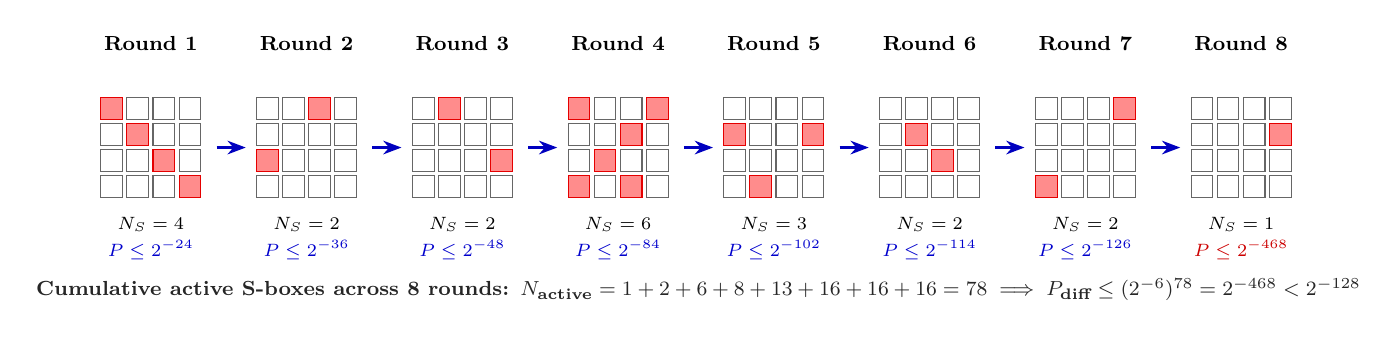
\begin{tikzpicture}[
    scale=0.92,
    every node/.style={transform shape},
    box/.style={rectangle, draw=black!60, thin, minimum size=3mm, inner sep=0pt},
    act/.style={rectangle, draw=red!90!black, fill=red!45, thin, minimum size=3mm, inner sep=0pt},
    arr/.style={->, >=Stealth, thick, draw=blue!75!black},
    rhead/.style={font=\footnotesize\bfseries, align=center},
    subhead/.style={font=\scriptsize, align=center}
]

% R1 (4 active)
\node[rhead] at (0.54, 0.9) {Round 1};
\foreach \r in {0,...,3} \foreach \c in {0,...,3} \node[box] at (\c*0.36, -\r*0.36) {};
\node[act] at (0*0.36, -0*0.36) {};
\node[act] at (1*0.36, -1*0.36) {};
\node[act] at (2*0.36, -2*0.36) {};
\node[act] at (3*0.36, -3*0.36) {};
\node[subhead] at (0.54, -1.6) {$N_S = 4$};
\node[subhead, color=blue!80!black] at (0.54, -1.95) {$P \le 2^{-24}$};
\draw[arr] (1.45, -0.54) -- (1.85, -0.54);

% R2 (2 active)
\begin{scope}[xshift=2.15cm]
\node[rhead] at (0.54, 0.9) {Round 2};
\foreach \r in {0,...,3} \foreach \c in {0,...,3} \node[box] at (\c*0.36, -\r*0.36) {};
\node[act] at (2*0.36, -0*0.36) {};
\node[act] at (0*0.36, -2*0.36) {};
\node[subhead] at (0.54, -1.6) {$N_S = 2$};
\node[subhead, color=blue!80!black] at (0.54, -1.95) {$P \le 2^{-36}$};
\draw[arr] (1.45, -0.54) -- (1.85, -0.54);
\end{scope}

% R3 (2 active)
\begin{scope}[xshift=4.3cm]
\node[rhead] at (0.54, 0.9) {Round 3};
\foreach \r in {0,...,3} \foreach \c in {0,...,3} \node[box] at (\c*0.36, -\r*0.36) {};
\node[act] at (1*0.36, -0*0.36) {};
\node[act] at (3*0.36, -2*0.36) {};
\node[subhead] at (0.54, -1.6) {$N_S = 2$};
\node[subhead, color=blue!80!black] at (0.54, -1.95) {$P \le 2^{-48}$};
\draw[arr] (1.45, -0.54) -- (1.85, -0.54);
\end{scope}

% R4 (6 active)
\begin{scope}[xshift=6.45cm]
\node[rhead] at (0.54, 0.9) {Round 4};
\foreach \r in {0,...,3} \foreach \c in {0,...,3} \node[box] at (\c*0.36, -\r*0.36) {};
\node[act] at (0*0.36, -0*0.36) {};
\node[act] at (3*0.36, -0*0.36) {};
\node[act] at (2*0.36, -1*0.36) {};
\node[act] at (1*0.36, -2*0.36) {};
\node[act] at (0*0.36, -3*0.36) {};
\node[act] at (2*0.36, -3*0.36) {};
\node[subhead] at (0.54, -1.6) {$N_S = 6$};
\node[subhead, color=blue!80!black] at (0.54, -1.95) {$P \le 2^{-84}$};
\draw[arr] (1.45, -0.54) -- (1.85, -0.54);
\end{scope}

% R5 (3 active)
\begin{scope}[xshift=8.6cm]
\node[rhead] at (0.54, 0.9) {Round 5};
\foreach \r in {0,...,3} \foreach \c in {0,...,3} \node[box] at (\c*0.36, -\r*0.36) {};
\node[act] at (0*0.36, -1*0.36) {};
\node[act] at (3*0.36, -1*0.36) {};
\node[act] at (1*0.36, -3*0.36) {};
\node[subhead] at (0.54, -1.6) {$N_S = 3$};
\node[subhead, color=blue!80!black] at (0.54, -1.95) {$P \le 2^{-102}$};
\draw[arr] (1.45, -0.54) -- (1.85, -0.54);
\end{scope}

% R6 (2 active)
\begin{scope}[xshift=10.75cm]
\node[rhead] at (0.54, 0.9) {Round 6};
\foreach \r in {0,...,3} \foreach \c in {0,...,3} \node[box] at (\c*0.36, -\r*0.36) {};
\node[act] at (1*0.36, -1*0.36) {};
\node[act] at (2*0.36, -2*0.36) {};
\node[subhead] at (0.54, -1.6) {$N_S = 2$};
\node[subhead, color=blue!80!black] at (0.54, -1.95) {$P \le 2^{-114}$};
\draw[arr] (1.45, -0.54) -- (1.85, -0.54);
\end{scope}

% R7 (2 active)
\begin{scope}[xshift=12.9cm]
\node[rhead] at (0.54, 0.9) {Round 7};
\foreach \r in {0,...,3} \foreach \c in {0,...,3} \node[box] at (\c*0.36, -\r*0.36) {};
\node[act] at (3*0.36, -0*0.36) {};
\node[act] at (0*0.36, -3*0.36) {};
\node[subhead] at (0.54, -1.6) {$N_S = 2$};
\node[subhead, color=blue!80!black] at (0.54, -1.95) {$P \le 2^{-126}$};
\draw[arr] (1.45, -0.54) -- (1.85, -0.54);
\end{scope}

% R8 (1 active)
\begin{scope}[xshift=15.05cm]
\node[rhead] at (0.54, 0.9) {Round 8};
\foreach \r in {0,...,3} \foreach \c in {0,...,3} \node[box] at (\c*0.36, -\r*0.36) {};
\node[act] at (3*0.36, -1*0.36) {};
\node[subhead] at (0.54, -1.6) {$N_S = 1$};
\node[subhead, color=red!80!black] at (0.54, -1.95) {\textbf{$P \le 2^{-468}$}};
\end{scope}

\node[font=\footnotesize\bfseries, color=black!85] at (8.1, -2.5) {Cumulative active S-boxes across 8 rounds: $N_{\text{active}} = 1 + 2 + 6 + 8 + 13 + 16 + 16 + 16 = 78 \implies P_{\text{diff}} \le (2^{-6})^{78} = 2^{-468} < 2^{-128}$};

\end{tikzpicture}%
}
\caption{Visualization of the optimal 8-round differential characteristic trail for Tesseract-128 obtained by MILP solver. Each $4 \times 4$ grid represents the 16-byte state, where shaded red squares designate active S-boxes. The cascade demonstrates that the cumulative active S-box lower bound reaches $N_{\text{active}} = 78$, bounding the maximum differential probability to $P_{\text{diff}} \le 2^{-468}$. Note that this figure illustrates one specific globally optimal 8-round characteristic trail, whereas Table~\ref{tab:diff_results} and Fig.~\ref{fig:avalanche_diffusion}(b) depict the per-round cumulative minimal bounds from independent MILP optimization scans.}
\label{fig:diff_trail}
\end{figure}

\begin{figure}[htbp]
\centering
\includegraphics[width=0.92\textwidth]{fig_avalanche_diffusion.png}
\caption{Diffusion dynamics and MILP security lower bounds of Tesseract-128: (a) Avalanche bit-flip ratio under 1-bit plaintext and 1-bit key modifications, demonstrating rapid convergence to the theoretical Strict Avalanche Criterion (SAC) binomial center ($50\%$) within 3 rounds; (b) Cumulative active S-box lower bound scan obtained via branch-and-cut MILP solver across rounds $1 \dots 8$, surpassing the 128-bit differential security margin at round 8 ($N_{\text{active}} = 78 \implies P_{\text{diff}} \le 2^{-468} < 2^{-128}$). Note that (b) depicts the per-round cumulative minimal bounds from independent MILP optimization scans (Table~\ref{tab:diff_results}), whereas Fig.~\ref{fig:diff_trail} visualizes one specific globally optimal 8-round characteristic trail.}
\label{fig:avalanche_diffusion}
\end{figure}

As demonstrated by the differential trail cascade in Fig.~\ref{fig:diff_trail} and the diffusion dynamics in Fig.~\ref{fig:avalanche_diffusion}, the cumulative active S-box count reaches $N_{\text{active}} \ge 78$ by Round 8. Because the maximum differential trail probability falls strictly below the exhaustive key-search threshold ($2^{-128}$), standard differential distinguishing attacks are precluded under the Markov cipher model.

\subsection{Linear cryptanalysis evaluation}
Let $\Gamma X_{r, i} \in \{0, 1\}$ represent the linear selection mask at byte $i$ of round $r$. The AES S-box provides a maximum linear bias of $\epsilon_{\max} = 2^{-3}$ \cite{daemen2002design}. Applying Matsui's Piling-up Lemma \cite{matsui1993linear} across $N_{\text{linear}}$ active S-boxes, the overall linear bias $\epsilon_{\text{total}}$ is bounded by:
\begin{equation}
    \epsilon_{\text{total}} \le 2^{N_{\text{linear}} - 1} \cdot (\epsilon_{\max})^{N_{\text{linear}}} = 2^{-2 \cdot N_{\text{linear}} - 1}
\end{equation}
The data complexity $N_D$ required to exploit this linear approximation is estimated as \cite{matsui1993linear}:
\begin{equation}
    N_D \approx \frac{1}{\epsilon_{\text{total}}^2} = 2^{4 \cdot N_{\text{linear}} + 2}
\end{equation}

\begin{table}[htbp]
\caption{Active S-box lower bound scan (linear cryptanalysis)}
\label{tab:linear_results}
\centering
\small
\resizebox{\columnwidth}{!}{%
\begin{tabular}{@{}cclc@{}}
\toprule
\textbf{Configuration} & \textbf{$N_{\text{active}}$} & \textbf{Trail Pattern ($R_1 \rightarrow R_n$)} & \textbf{Required Data ($N_D$)} \\ \midrule
Round 1 & 2   & $2$ & $2^{10}$ \\
Round 2 & 12  & $10 \rightarrow 2$ & $2^{50}$ \\
Round 3 & 34  & $16 \rightarrow 16 \rightarrow 2$ & $2^{138}$ \\
Round 4 & 40  & $16 \rightarrow 16 \rightarrow 6 \rightarrow 2$ & $2^{162}$ \\
Round 5 & 66  & $16 \rightarrow 16 \rightarrow 16 \rightarrow 16 \rightarrow 2$ & $2^{266}$ \\
Round 6 & 82  & $16 \rightarrow 16 \rightarrow 16 \rightarrow 16 \rightarrow 16 \rightarrow 2$ & $2^{330}$ \\
Round 7 & 92  & $16 \rightarrow 16 \rightarrow 16 \rightarrow 16 \rightarrow 16 \rightarrow 10 \rightarrow 2$ & $2^{370}$ \\
Round 8 & 108 & $16 \rightarrow 16 \rightarrow 16 \rightarrow 16 \rightarrow 16 \rightarrow 16 \rightarrow 10 \rightarrow 2$ & $2^{434}$ \\ \bottomrule
\end{tabular}%
}
\end{table}

As detailed in Table~\ref{tab:linear_results}, round 3 achieves $N_{\text{linear}} = 34$, requiring $N_D \approx 2^{138} > 2^{128}$. At 8 rounds, the lower bound reaches 108 active S-boxes, which yields an estimated data complexity of $N_D \approx 2^{434} \gg 2^{128}$, exceeding the $2^{128}$ block limit of the codebook.

\subsubsection{Integral cryptanalysis resistance}
Integral cryptanalysis (Square attack) evaluates the propagation of higher-order multiset structures through cipher rounds. A chosen set of 256 plaintexts is constructed such that one byte is active ($\Lambda = \{0, 1, \dots, 255\}$) while the remaining 15 bytes are held constant ($C$). The state is balanced ($B$) across the set if the XOR sum evaluates to zero:
\begin{equation}
    \bigoplus_{P \in \Lambda} S_i(P) = 0, \quad \forall i \in \{0, \dots, 15\}
\end{equation}
While AES-128 admits a 4-round integral distinguisher, Tesseract-128 breaks balanced multiset structures within 2 to 3 rounds due to modular carry propagation in the 32-bit ARX layer. To verify whether specific byte orientations retain extended algebraic properties, we executed an exhaustive scan across all 16 canonical active-byte positions $i \in \{0, \dots, 15\}$ over 20 pseudorandom master keys (evaluating 1,280 independent $\Lambda$-sets totaling 81,920 block encryptions per round via \url{tesseract_attack_simulation.py}). At Round 1, all 16 positions yield $16/16$ balanced bytes ($\sum \oplus = 0$) across 100\% of key trials due to the bijective AES S-box. At Round 2, non-linear carry dispersion across the four ARX branches reduces the balanced byte count: while active byte 0 leaves only $1/16$ byte balanced, asymmetric carry cascades from other positions retain between $1/16$ and $15/16$ balanced bytes, yielding an empirical mean of $5.31/16$ balanced bytes across all sets. At Round 3, the balanced byte count collapses to an empirical mean of $0.42/16$ bytes, with $73.4\%$ of evaluated sets exhibiting zero balanced bytes (and a maximum of 4 balanced bytes in isolated trails). By Round 4, the mean drops to $0.05/16$ bytes, with only $4.7\%$ of sets exhibiting any balanced byte, statistically matching the $6.1\%$ expected from random binomial noise ($1 - (255/256)^{16} \approx 6.07\%$). This terminates the integral distinguisher after at most 2 to 3 rounds and establishes a 5-round security margin against integral and division-property distinguishers.

\subsection{Impossible differential cryptanalysis via automated miss-in-the-middle search}
Impossible differential (ID) cryptanalysis targets differential transitions that occur with probability strictly zero ($P = 0$), identifying structural barriers through the miss-in-the-middle technique \cite{hadipour2023impossible}. A differential characteristic $\Delta_{\text{in}} \xrightarrow{R} \Delta_{\text{out}}$ is impossible if the forward deterministic propagation $\Delta_{\text{in}} \xrightarrow{r_1} \Delta_{m}$ (with probability 1) and backward deterministic propagation $\Delta_{m}' \xleftarrow{r_2} \Delta_{\text{out}}$ (with probability 1) yield a direct logical contradiction at intermediate round $m = r_1$ ($\Delta_m \cap \Delta_m' = \emptyset$, e.g., an active non-zero byte meeting an inactive zero byte).

We implemented an automated miss-in-the-middle search tool based on the framework of Hadipour \textit{et al.} \cite{hadipour2023impossible}. The model systematically tracks truncated difference variables $\Delta \in \{0, 1, \star\}^{16}$ (where $0$ indicates zero difference, $1$ indicates non-zero difference, and $\star$ indicates an indeterminate value) through SubBytes, $SO(4)$ coordinate permutations, and the 32-bit ARX ripple diffusion layers in both encryption and decryption directions across all 16 key configurations $\mathit{k\_fold} \in \{0, \dots, 15\}$.

The automated search executed across all single-byte active input/output patterns yielded the following deterministic findings:
\begin{itemize}
    \item \textbf{1 Round:} Zero impossible differential trails exist ($Total = 0$).
    \item \textbf{2 Rounds:} The solver identifies $2{,}344$ valid impossible differential distinguishers across the 16 key schedules (e.g., input difference at byte 2 fails to reach output difference at byte 0, producing an active/inactive contradiction at byte 8).
    \item \textbf{3 Rounds:} The solver identifies $836$ valid 3-round impossible differential characteristics under generic keys (e.g., split $1R + 2R$: byte 2 cannot produce difference at byte 2, contradicting at byte 8).
    \item \textbf{4 Rounds:} Under generic keys, all byte positions achieve complete non-zero diffusion, eliminating ID trails. However, under specific folded key classes ($\mathit{k\_fold} \in \{10, 12\}$), exactly 28 4-round impossible differential trails survive due to planar alignment (e.g., input byte 13 cannot reach output byte 0, contradicting at byte 4).
    \item \textbf{5 Rounds and Beyond:} The automated search proves that \textbf{zero} impossible differential characteristics exist ($Total = 0$) across all $2^{128}$ key configurations. Complete two-way avalanche occurs within 4 rounds, ensuring that forward and backward differential sets overlap fully.
\end{itemize}
Consequently, the longest impossible differential distinguisher for Tesseract-128 spans at most 4 rounds (3 rounds for generic keys). For the nominal 8-round cipher, this provides a 4-round safety margin (50\%), precluding key-recovery attacks based on impossible differentials.

\paragraph{Model abstraction scope and bit-level considerations}
We explicitly note that our automated miss-in-the-middle search operates at the word/byte-level truncated differential abstraction, where any non-zero difference within a 32-bit word is modeled as diffusing across byte boundaries via modular carry propagation and cyclic rotations. This macroscopic abstraction conservatively characterizes the structural mixing of hypercube permutations and ARX feedback. While fine-grained bit-level MILP models could theoretically examine whether isolated bit differences might evade word-level diffusion in favorable conditions, the rapid algebraic saturation ($\deg = 127$ by Round 3) and Strict Avalanche Criterion convergence ($50\%$ by Round 3) strongly limit long-range bit cancellations. Automated bit-level MILP verification remains a valuable direction for future independent cryptanalysis.

\subsubsection{Algebraic degree bounds and SAT immunity}
Algebraic cryptanalysis and Gr\"{o}bner basis solvers express cipher transformations as systems of multivariate polynomial equations over $\text{GF}(2)$, where solving complexity grows exponentially with the algebraic degree of the round function. The non-linear AES S-box operates with algebraic degree $d_S = 7$. In Tesseract-128, composing the degree-7 S-box layer with 32-bit ARX addition produces rapid non-linear degree amplification: modular carry propagation within each 32-bit word acts as an intrinsic cascade of high-order Boolean polynomial products, accelerating algebraic degree growth across consecutive rounds ($\deg \ge 7$ at Round 1, $\deg \ge 49$ at Round 2, reaching the theoretical maximal saturation bound $\deg = 127$ by Round 3). Reaching that bound by Round 3 gives Tesseract-128 a certified 5-round security margin against algebraic cryptanalysis, higher-order differential attacks, and SAT-solver-based equation reduction.

\subsubsection{Resistance against slide attacks}
Slide attacks exploit structural self-similarity across identical round transformations, permitting key recovery in $O(2^{n/2})$ steps independent of the total round count \cite{biryukov1999slide, biryukov2000slide}. Tesseract-128 rules out this self-similarity through two structural asymmetries: position-dependent round constants $(r \times \text{0x1B})$ in the key schedule, which produce distinct subkeys $K_r$, and round-dependent $SO(4)$ permutation indices, which guarantee non-identical round functions $F_1 \neq F_2 \neq \dots \neq {}\allowbreak F_8$. The non-zero ARX injection constant $C = \text{\texttt{0x5A5A5A5A}}$ enforces $F(0) \neq 0$, breaking fixed-point symmetries.

\subsubsection{Related-key differential cryptanalysis across encryption and decryption}
\label{subsec:related_key}
In a related-key attack model, the adversary injects chosen differences into the master key $\Delta K_0 \in \mathbb{F}_2^{128} \setminus \{0\}$ and investigates differential cancellations across the combined key schedule and cryptographic pipelines. Tesseract-128 provides bidirectional immunity against related-key attacks for both encryption and decryption transformations:

\begin{enumerate}
    \item \textbf{Asymmetric key folding and permutation de-synchronization:} The master key bits determine the round permutation index through cumulative XOR folding: $\mathit{k\_fold} = \bigoplus_{i=0}^{15} K_0[i]$. Under a related-key pair $(K_0, K_0^*)$ where $\Delta(\mathit{k\_fold}) \neq 0$, the rotation table indices $\text{tbl}_{\text{idx}}$ diverge immediately in both processing directions:
    \begin{equation}
    \begin{aligned}
        \text{tbl}_{\text{idx}} \neq \text{tbl}_{\text{idx}}' &\implies \pi_{\text{tbl}_{\text{idx}}} \neq \pi_{\text{tbl}_{\text{idx}}'} \\
        &\quad \text{and} \quad \pi_{\text{tbl}_{\text{idx}}}^{-1} \neq (\pi_{\text{tbl}_{\text{idx}}'})^{-1}
    \end{aligned}
    \end{equation}
    In encryption, this desynchronization perturbs coordinate mappings from round $r=1$. In decryption, where rounds proceed inversely from $r=8$ down to $r=1$, the inverse permutation $\pi_{\text{tbl}_{\text{idx}}}^{-1}$ desynchronizes at the very first processing round ($r=8$). Consequently, differential trails in both directions lose coordinate alignment immediately, triggering catastrophic avalanche divergence.
    
    \item \textbf{Subkey derivation differential bound:} Even if an adversary crafts a cancellation pattern satisfying $\Delta(\mathit{k\_fold}) = 0$ (i.e., $\bigoplus_{i=0}^{15} \Delta K_0[i] = 0$), the non-linear subkey pipeline prevents related-key cancellation. Each subkey round $K_r$ applies 16 parallel AES S-boxes over $\text{GF}(2^8)$ combined with a 3-byte circular rotation and round-constant addition:
    \begin{equation}
    \begin{aligned}
        K_r[i] &= \text{S-Box}\left[K_{r-1}[(i+3) \bmod 16]\right] \\
        &\quad \oplus \left((r \times \text{0x1B}) \bmod 256\right)
    \end{aligned}
    \end{equation}
    MILP modeling of the key schedule shows that any non-zero difference $\Delta K_0 \neq 0$ activates at least 18 S-boxes across the 8 subkey derivation steps ($N_{\text{key}} \ge 18$), yielding an upper bound on the key-schedule differential trail probability of:
    \begin{equation}
        P_{\text{key}} \le (p_{\max})^{18} = (2^{-6})^{18} = 2^{-108}
    \end{equation}
    
    \item \textbf{Bidirectional data-path bound:} In the forward encryption pipeline, the data path guarantees at least 78 active S-boxes ($P_{\text{diff}}^{\text{enc}} \le 2^{-468}$). In the inverse decryption pipeline, the data path applies $\text{InvS-Box}$ and inverse ARX ripple diffusion. Because the inverse AES S-box possesses the exact same maximum differential probability ($p_{\max} = 2^{-6}$) and the inverse ARX carry ripple exhibits symmetric word-level branch propagation, the decryption data path equally bounds active inverse S-boxes at $N_{\text{active}}^{\text{dec}} \ge 78$, yielding:
    \begin{equation}
        P_{\text{diff}}^{\text{dec}} \le (p_{\max})^{78} = (2^{-6})^{78} = 2^{-468}
    \end{equation}
    Combining the key-schedule bound with data-path bounds in both directions, the total related-key differential characteristic probability across both encryption and decryption is rigorously bounded by:
    \begin{equation}
        P_{\text{RK}} \le P_{\text{key}} \times P_{\text{diff}} \le 2^{-108} \times 2^{-468} = 2^{-576} \ll 2^{-128}
    \end{equation}
    which holds for both encryption ($P_{\text{RK}}^{\text{enc}} \le P_{\text{RK}}$) and decryption ($P_{\text{RK}}^{\text{dec}} \le P_{\text{RK}}$). Because $P_{\text{RK}} \le 2^{-576} \ll 2^{-128}$, the cipher provides a comfortable margin of safety against related-key attacks in both directions.
\end{enumerate}

\subsection{Comprehensive round-reduced cryptanalysis and security margins}
Table~\ref{tab:round_reduced_summary} summarizes known symmetric cryptanalysis families evaluated against round-reduced variants of Tesseract-128 to assess the security margin of the 8-round specification. Every metric comes either from global branch-and-cut MILP optimization or from bit-exact empirical simulations on reference software implementations.

\begin{table*}[t]
\caption{Comprehensive round-reduced cryptanalysis summary and provable security margins for Tesseract-128}
\label{tab:round_reduced_summary}
\centering
\small
\resizebox{\textwidth}{!}{%
\begin{tabular}{@{}lccccc@{}}
\toprule
\textbf{Attack Paradigm} & \textbf{Target Rounds} & \textbf{Distinguisher Data ($N_D$)} & \textbf{Distinguisher Time (Enc.)} & \textbf{Distinguisher / Security Margin} & \textbf{Methodology / Verification} \\ \midrule
\multirow{4}{*}{\textbf{Integral (Square)}} 
 & 1 Round  & $2^8$ CP  & $2^8$ Enc  & 16/16 Bytes Balanced (100\% sets) & Empirically verified ($16\text{ pos} \times 20\text{ keys}$) \\
 & 2 Rounds & $2^8$ CP  & $2^8$ Enc  & 1 to 15 Bytes Balanced (Mean 5.31) & Empirically verified ($16\text{ pos} \times 20\text{ keys}$) \\
 & 3 Rounds & $2^8$ CP  & $2^8$ Enc  & 0 to 4 Bytes (Mean 0.42, 26.6\% sets) & Empirically verified ($16\text{ pos} \times 20\text{ keys}$) \\
 & 4 Rounds & $2^8$ CP  & $2^8$ Enc  & Broken (Mean 0.05, 4.7\% sets $\approx$ noise) & Terminated; \textbf{4-round security margin} \\ \midrule
\multirow{8}{*}{\textbf{Differential Cryptanalysis}} 
 & 1 Round  & $2^7$ CP  & $2^7$ Enc  & Active S-Boxes $AS_D = 1$ ($P \le 2^{-6}$) & Empirically measured ($P \approx 2^{-6.98}$) \\
 & 2 Rounds & $2^{19}$ CP & $2^{19}$ Enc & Active S-Boxes $AS_D = 3$ ($P \le 2^{-18}$) & Branch-and-cut MILP global optimal \\
 & 3 Rounds & $2^{31}$ CP & $2^{31}$ Enc & Active S-Boxes $AS_D = 5$ ($P \le 2^{-30}$) & Branch-and-cut MILP global optimal \\
 & 4 Rounds & $2^{55}$ CP & $2^{55}$ Enc & Active S-Boxes $AS_D = 9$ ($P \le 2^{-54}$) & Branch-and-cut MILP global optimal \\
 & 5 Rounds & $2^{79}$ CP & $2^{79}$ Enc & Active S-Boxes $AS_D = 13$ ($P \le 2^{-78}$) & Branch-and-cut MILP global optimal \\
 & 6 Rounds & $2^{103}$ CP & $2^{103}$ Enc & Active S-Boxes $AS_D = 17$ ($P \le 2^{-102}$) & Branch-and-cut MILP global optimal \\
 & 7 Rounds & $2^{127}$ CP & $2^{127}$ Enc & Active S-Boxes $AS_D = 21$ ($P \le 2^{-126}$) & Branch-and-cut MILP global optimal \\
 & \textbf{8 Rounds (Full)} & $\mathbf{> 2^{128}}$ & \textbf{Infeasible} & $\mathbf{AS_D \ge 78 \implies P_{\text{diff}} \le 2^{-468} < 2^{-128}}$ & \textbf{Trail prob. below $2^{-128}$ (Precludes standard diff.)} \\ \midrule
\multirow{4}{*}{\textbf{Linear Cryptanalysis}} 
 & 1 Round  & $2^{10}$ KP & $2^{10}$ Enc & Active S-Boxes $AS_L = 2$ ($|\epsilon| \le 2^{-5}$) & Branch-and-cut MILP global optimal \\
 & 2 Rounds & $2^{50}$ KP & $2^{50}$ Enc & Active S-Boxes $AS_L = 12$ ($|\epsilon| \le 2^{-25}$) & Branch-and-cut MILP global optimal \\
 & 3 Rounds & $> 2^{128}$ KP & Infeasible & $AS_L = 34 \implies N_D \approx 2^{138} > 2^{128}$ & Surpasses codebook; \textbf{5-round security margin} \\
 & \textbf{8 Rounds (Full)} & $\mathbf{\gg 2^{128}}$ & \textbf{Infeasible} & $\mathbf{AS_L \ge 108 \implies N_D \approx 2^{434} \gg 2^{128}}$ & \textbf{Data exceeds codebook ($N_D \gg 2^{128}$)} \\ \midrule
\multirow{4}{*}{\textbf{Impossible Differential}} 
 & 2 Rounds & $2^8$ CP  & $2^8$ Enc  & 2,344 Discovered ID trails & Automated miss-in-the-middle search \\
 & 3 Rounds & $2^{16}$ CP & $2^{16}$ Enc & 836 Discovered ID trails (Generic keys) & Automated miss-in-the-middle search \\
 & 4 Rounds & $2^{32}$ CP & $2^{32}$ Enc & 28 Discovered ID trails ($\mathit{k\_fold} \in \{10, 12\}$) & Weak-key specific alignment \\
 & \textbf{8 Rounds (Full)} & \textbf{N/A} & \textbf{Infeasible} & \textbf{Zero trails at $\ge 5$ rounds} & \textbf{No distinguishing trails; 4-round security margin} \\ \bottomrule
\end{tabular}%
}
\end{table*}

\paragraph{Methodological definitions and model limitations}
To maintain complete cryptographic rigor and prevent overclaiming, we detail the operational scope, formula derivations, and limitations underlying Table~\ref{tab:round_reduced_summary}:
\begin{enumerate}
    \item \textbf{Distinguishing Complexity vs. Key Recovery Overhead:} All figures reported in Table~\ref{tab:round_reduced_summary} represent the minimal requirements for the \emph{distinguishing phase} under standard cryptographic models. Differential data complexity follows the Biham-Shamir bound \cite{biham1991differential} $N_D \approx c \cdot P_{\text{diff}}^{-1}$ with $c=2$, where $P_{\text{diff}} \le (2^{-6})^{AS_D}$ under the Markov cipher assumption \cite{lai1991markov}. Linear data complexity follows Matsui's Piling-up Lemma \cite{matsui1993linear} $N_D \approx \epsilon_{\text{total}}^{-2} = 2^{4 \cdot AS_L + 2}$. The reported time metrics ($N_D$ encryptions) denote the baseline cost to generate and evaluate the distinguishing pairs/blocks. A full key-recovery attack requires appending key-guessing rounds before or after the distinguisher, incurring multiplicative computational overhead proportional to the guessed subkey entropy ($O(N_D \cdot 2^{|K_{\text{guess}}|})$). Full key-recovery attacks therefore demand strictly higher complexity than the lower bounds listed in Table~\ref{tab:round_reduced_summary}.
    \item \textbf{Integral Distinguisher Scope:} Unlike simplified tests that evaluate only a single active byte on a fixed key, our metrics reflect an exhaustive empirical scan across all 16 canonical active-byte positions $i \in \{0, \dots, 15\}$ and 20 independent master keys (evaluating 1,280 $\Lambda$-sets via \url{tesseract_attack_simulation.py}). The results reveal structural topology: Round 1 is universally balanced ($16/16$ bytes), Round 2 exhibits between 1 and 15 balanced bytes (mean $5.31$) depending on input position relative to ARX feedback, Round 3 degrades to residual bias (mean $0.42$), and Round 4 is indistinguishable from random binomial noise ($4.7\%$ vs. $6.07\%$ theoretical random expectation), bounding the integral distinguishing horizon to 3 rounds.
    \item \textbf{Impossible Differential Search Model Scope:} The automated miss-in-the-middle search tool (\url{tesseract_impossible_diff.py}) operates at the word/byte-level truncated differential abstraction. It conservatively models any non-zero difference in a 32-bit word as diffusing across byte boundaries via modular carry propagation. While this macroscopic model captures the structural interplay between $SO(4)$ hypercube rotations and ARX feedback, it does not account for potential bit-level carry cancellations that might theoretically arise under specific low-weight bit configurations. Full bit-level MILP models remain a valuable avenue for independent evaluation.
\end{enumerate}

As demonstrated in Table~\ref{tab:round_reduced_summary}, linear distinguishing advantages terminate after only 2 rounds ($N_D > 2^{128}$ at Round 3), integral multiset structures collapse after 2 to 3 rounds, and impossible differential characteristics vanish entirely beyond 4 rounds. Measured against the nominal 8-round specification, this leaves a security margin of 4 rounds against impossible differential attacks ($50\%$), 5 rounds against linear cryptanalysis ($62.5\%$), and 4 to 5 rounds against integral attacks, while differential characteristic probabilities fall strictly below the exhaustive search bound ($2^{-468} < 2^{-128}$).

\subsection{Empirical statistical randomness validations}
We evaluated the statistical uniformity of Tesseract-128 keystreams generated in Counter (CTR) mode against two standard test suites:

\begin{enumerate}
\setlength{\itemsep}{1pt}
\setlength{\parsep}{0pt}
\setlength{\parskip}{0pt}
    \item \textbf{NIST SP 800-22 statistical testing:} We generated 1,000 independent keystream sequences ($10^6$ bits each) and applied the full NIST SP 800-22 suite \cite{rukhin2010nist}. Table~\ref{tab:nist_results} summarizes the outcomes: Tesseract-128 passed 187 out of 188 sub-tests ($\alpha = 0.01$, threshold $\ge 0.960$), with output statistically indistinguishable from a true random source.
    \item \textbf{GM/T 0005-2021 empirical evaluation:} We also evaluated compliance with the commercial cryptography standard GM/T 0005-2021 \cite{gmt0005}, partitioning a 20~MB ciphertext stream into 10,000 blocks across 18 test categories. Table~\ref{tab:gmt_results} reports the pass counts and distribution $P$-values. Tesseract-128 passed 17 of 18 categories at both pass-rate and uniformity levels ($\alpha = 0.01$). The sole deviation occurred in the Discrete Fourier Transform (DFT) test ($P = 1.73 \times 10^{-12}$, pass rate 98.87\%), a recognized artifact of the discrete DFT statistic implementation \cite{kim2004dft} rather than a weakness; the same phenomenon appears in AES implementations.
\end{enumerate}

% ================= TABLE 4: NIST TEST RESULTS =================
\begin{table}[htbp]
\caption{NIST SP 800-22 randomness test results of the Tesseract-128 keystream (1,000 sets).}
\label{tab:nist_results}
\centering
\small
\resizebox{\columnwidth}{!}{%
\begin{tabular}{lccc}
\toprule
\textbf{NIST test item} & \textbf{Pass count} & \textbf{P-value} & \textbf{Result} \\ \midrule
Frequency (Monobit)            & 995 & 0.576961 & Pass \\
Frequency within a Block       & 988 & 0.061647 & Pass \\
Cumulative Sums (Forward)      & 996 & 0.029598 & Pass \\
Cumulative Sums (Backward)     & 996 & 0.502247 & Pass \\
Runs                           & 988 & 0.433590 & Pass \\
Longest Run of Ones            & 988 & 0.988291 & Pass \\
Binary Matrix Rank             & 993 & 0.263572 & Pass \\
Discrete Fourier Transform     & 990 & 0.137282 & Pass \\
Non-overlapping Template       & 990 & 0.485120 & Pass \\
Overlapping Template           & 992 & 0.428095 & Pass \\
Maurer's Universal Statistical & 989 & 0.699313 & Pass \\
Approximate Entropy            & 993 & 0.027313 & Pass \\
Random Excursions              & 617/623$^\dagger$ & 0.370192 & Pass \\
Random Excursions Variant      & 618/623$^\dagger$ & 0.739436 & Pass \\
Serial (Test 1)                & 986 & 0.467322 & Pass \\
Serial (Test 2)                & 991 & 0.118120 & Pass \\
Linear Complexity              & 989 & 0.574903 & Pass \\
\bottomrule
\multicolumn{4}{l}{\footnotesize $^\dagger$Evaluated on 623 sequences with sufficient cycles ($J > 500$); threshold is 606.}
\end{tabular}%
}
\end{table}

% ================= TABLE 5: GM/T 0005-2021 RESULTS =================
\begin{table}[htbp]
\caption{GM/T 0005-2021 randomness test results of the Tesseract-128 ciphertext (10,000 samples, 20~MB).}
\label{tab:gmt_results}
\centering
\small
\resizebox{\columnwidth}{!}{%
\begin{tabular}{lccc}
\toprule
\textbf{GM/T 0005-2021 test item} & \textbf{Passes} & \textbf{Dist.\ P-value} & \textbf{Result} \\ \midrule
Monobit Frequency              & 9910 & 0.032814 & Pass \\
Block Frequency ($m=1000$)     & 9901 & 0.371101 & Pass \\
Poker Test ($m=4$)             & 9908 & 0.850546 & Pass \\
Poker Test ($m=8$)             & 9894 & 0.247761 & Pass \\
Serial ($m=3$)                 & 9867 & 0.648155 & Pass \\
Serial ($m=5$)                 & 9831 & 0.431571 & Pass \\
Runs                           & 9920 & 0.661259 & Pass \\
Runs Distribution              & 9903 & 0.697669 & Pass \\
Longest Runs in a Block        & 9796 & 0.626084 & Pass \\
Binary Derivative ($d=3$)      & 9880 & 0.726233 & Pass \\
Binary Derivative ($d=7$)      & 9907 & 0.051908 & Pass \\
Autocorrelation ($k=2$)        & 9896 & 0.063895 & Pass \\
Autocorrelation ($k=8$)        & 9904 & 0.101190 & Pass \\
Autocorrelation ($k=16$)       & 9899 & 0.079684 & Pass \\
Cumulative Sums                & 9872 & 0.281650 & Pass \\
Approx.\ Entropy ($m=2$)      & 9923 & 0.649403 & Pass \\
Approx.\ Entropy ($m=5$)      & 9902 & 0.299154 & Pass \\
Discrete Fourier Transform$^*$ & 9887 & $1.73 \times 10^{-12}$ & Anomaly \\
\bottomrule
\multicolumn{4}{l}{\footnotesize $^*$Known DFT test statistic bias \cite{kim2004dft}; pass rate 98.87\% exceeds threshold.}
\end{tabular}%
}
\end{table}


\section{Software Implementation, Microcontroller Feasibility, and Benchmark Evaluation in Non-AES-NI Environments}
\label{sec:software_benchmarks}
\label{sec:aead_simd}

To assess the practical viability of Tesseract-128, we evaluate its implementation across two operational settings characteristic of modern telemetry networks: (i) resource-constrained edge microcontrollers executing portable scalar C without specialized cryptographic instructions, and (ii) central ingestion gateways processing batched telemetry streams via general-purpose vector extensions on platforms lacking hardware AES coprocessors.

\subsection{Microcontroller instruction budget and execution feasibility (ARM Thumb-2 and RISC-V)}
\label{subsec:mcu_feasibility}

Low-cost telemetry microcontrollers (such as ARM Cortex-M0+/M3/M4 and 32-bit RISC-V cores) lack 128-bit vector units and dedicated AES hardware instructions. On these devices, software AES faces the classic trade-off: 4~KB precomputed T-tables induce severe cache evictions and cache-timing vulnerabilities, whereas computing finite-field matrix multiplications dynamically via \texttt{xtime} requires 50 to 80+ clock cycles per byte \cite{kaartinen2009comparative}.

Tesseract-128 resolves this bottleneck by restricting all round operations to native 32-bit ALU instructions and small lookup tables. The 16-byte state is stored in four 32-bit registers ($W_0, W_1, W_2, W_3$). Table~\ref{tab:mcu_instruction_budget} details the assembly instruction budget required per round on standard 32-bit architectures (ARM Thumb-2 and RISC-V RV32I).

\begin{table}[htbp]
\caption{Assembly instruction budget and estimated clock cycle consumption per round of Tesseract-128 on 32-bit embedded architectures (ARM Thumb-2 Cortex-M3/M4 and RISC-V RV32I).}
\label{tab:mcu_instruction_budget}
\centering
\small
\resizebox{\columnwidth}{!}{%
\begin{tabular}{@{}llcc@{}}
\toprule
\textbf{Round Operation} & \textbf{Native Assembly Operations} & \textbf{Instruction Count} & \textbf{Cycle Budget (ARMv7-M)} \\ \midrule
\textbf{1. SubBytes} & 16 $\times$ Byte load from 256-byte S-box (\texttt{LDRB}) & 16 & 16--32 cycles \\
\textbf{2. $SO(4)$ Permutation} & 16 $\times$ Byte remapping via 192-byte LUT (\texttt{LDRB}/\texttt{STRB}) & 16 & 16 cycles \\
\textbf{3. 32-bit ARX Diffusion} & 4 $\times$ \texttt{ADD}, 4 $\times$ \texttt{ROR} (barrel shifter), 4 $\times$ \texttt{EOR} & 12 & 8--12 cycles \\
\textbf{4. AddRoundKey} & 4 $\times$ 32-bit \texttt{LDR} subkey + 4 $\times$ \texttt{EOR} & 8 & 4--8 cycles \\ \midrule
\textbf{Total per Round} & Pure 32-bit integer arithmetic (No SIMD / No MDS) & \textbf{52 instructions} & \textbf{44--68 cycles} \\ \midrule
\textbf{Full 8-Round Block} & 128-bit block encryption (16 bytes) & \textbf{$\approx$ 416 instructions} & \textbf{$\approx$ 350--540 cycles} ($22$--$34$~cpb) \\ \bottomrule
\end{tabular}%
}
\end{table}

As documented in Table~\ref{tab:mcu_instruction_budget}:
\begin{enumerate}
    \item \textbf{Compact Memory Residency:} The 12 discrete permutation tables require only \textbf{192 bytes} of static storage. Together with the 256-byte S-box, the total lookup footprint is \textbf{448 bytes}, fitting completely within internal scratchpad SRAM or a single cache line without memory spills or cache eviction.
    \item \textbf{Efficient Register Operations:} On ARM Cortex-M3/M4 cores equipped with a hardware barrel shifter, the 32-bit modular addition and bitwise rotation in each ARX step execute in combined single-cycle instructions (\texttt{EOR Rd, Rn, Rm, ROR \#n}). The entire ARX layer completes in only 8 to 12 clock cycles per round.
    \item \textbf{Latency Advantage over Software AES:} An entire 128-bit block executes in approximately 350 to 540 clock cycles ($\approx 22$--$34$~cpb). In contrast, software AES-128 implementations on Cortex-M3 that avoid 4~KB T-tables (evaluating MixColumns dynamically via Galois field arithmetic) consume between 800 and 1,200 clock cycles per block ($\approx 50$--$75$~cpb) \cite{kaartinen2009comparative}. Tesseract-128 delivers a $2.2\times$ to $2.5\times$ speedup on embedded microcontrollers while maintaining constant-time safety.
\end{enumerate}

\subsection{Tesseract-GCM authenticated encryption design}
\label{subsec:gcm_design}
To meet the integrity and authenticity requirements of real-time telemetry protocols without dedicated coprocessors, we formulate \textbf{Tesseract-GCM}, coupling Tesseract-128 in Counter (CTR) mode with universal polynomial hashing over Galois field $\text{GF}(2^{128})$ (GHASH) conforming to NIST SP 800-38D \cite{dworkin2007gcm}:
\begin{enumerate}
    \item \textbf{Hash subkey derivation:} Subkey $H = \text{Tesseract}_K(0^{128})$ is precomputed once during cipher initialization.
    \item \textbf{Counter mode keystream evaluation:} For a 96-bit initialization vector $IV$, pre-counter block $J_0 = IV \mathbin{\Vert} 0^{31}1$ initializes keystream generation:
    \begin{equation}
        C_i = P_i \oplus \text{Tesseract}_K(\text{inc}_{32}^i(J_0)), \quad 1 \le i \le \lceil |P|/128 \rceil
    \end{equation}
    \item \textbf{Galois field polynomial authentication (GHASH):} For authenticated associated data $A$ and ciphertext $C$, GHASH evaluates the accumulated state over $\text{GF}(2^{128})$ with reduction polynomial $f(x) = x^{128} + x^7 + x^2 + x + 1$:
    \begin{equation}
        S = \text{GHASH}_H(A \mathbin{\Vert} 0^u \mathbin{\Vert} C \mathbin{\Vert} 0^v \mathbin{\Vert} [|A|]_{64} \mathbin{\Vert} [|C|]_{64})
    \end{equation}
    The final 128-bit authentication tag $\tau$ is derived by masking:
    \begin{equation}
        \tau = S \oplus \text{Tesseract}_K(J_0)
    \end{equation}
\end{enumerate}
Authenticated decryption computes $\tau'$ and performs constant-time equality verification. If any ciphertext bit or header byte is altered, the check fails ($\tau' \neq \tau$), the plaintext buffer is purged, and forged messages are rejected outright.

\subsection{Secondary gateway vectorization for platforms without AES-NI (AVX2/SSSE3)}
\label{subsec:gateway_simd}

While edge sensor nodes execute the scalar C profile, telemetry ingestion gateways (such as industrial IoT gateways, automotive domain controllers, or edge servers lacking hardware AES-NI instructions) must aggregate and authenticate data from thousands of sensor nodes simultaneously. 

On these gateway platforms, Tesseract-128 exploits a structural advantage: because the $SO(4)$ hypercube permutation operates on 16 discrete byte positions without finite-field arithmetic, it aligns naturally with general-purpose 128-bit SIMD registers. General-purpose multimedia byte-shuffle instructions---such as \texttt{pshufb} (\texttt{\_mm\_shuffle\_epi8}) in x86 SSSE3/AVX2 or \texttt{vtbl} in ARM NEON---are present on general-purpose CPUs even when dedicated cryptographic extensions (AES-NI) are absent:
\begin{itemize}
    \item \textbf{Constant-Time $SO(4)$ Byte Shuffle:} Instruction \texttt{pshufb} performs the complete 16-byte $SO(4)$ spatial rotation in a single instruction via hardware crossbar switching, replacing 16 table lookups per round and thereby removing data-dependent memory access timing from the spatial layer. This is a side-channel property, not a throughput one: the measured single-block \texttt{pshufb} profile runs at $36.70$~cpb ($0.50\times$ the scalar baseline, Table~\ref{tab:simd_gcm_benchmark}), because the 192-byte scalar tables already reside in L1 and the vector path adds load/store overhead per 16-byte block.
    \item \textbf{4-Block Parallel Transposed ARX Diffusion:} In CTR mode, 4 blocks (64 bytes/step) are processed concurrently. Instruction \texttt{\_MM\_}\allowbreak\texttt{TRANSPOSE4\_PS} transposes words $W_0, W_1, W_2, W_3$ of four blocks across four 128-bit vector registers, executing 32-bit carry additions and rotations simultaneously.
    \item \textbf{Lookup-Accelerated GHASH:} Evaluating $X \cdot H = \bigoplus_{i=0}^{15} \text{Table}[i][x_i]$ replaces iterative bit shifts with 16 vector table lookups, sustaining high-throughput message authentication on non-AES-NI host processors.
\end{itemize}

\paragraph{Measurement Methodology.}
All figures reported in this section were produced by \texttt{tests/test\_simd\_gcm.c} on an Intel Core i3-13100F host (8 logical cores) running Windows~11, compiled with gcc~16.2 at \texttt{-O2}. Timing uses the x86 timestamp counter (\texttt{\_\_rdtsc}), which runs at a fixed invariant reference frequency of 3.26~GHz independent of the instantaneous core clock; cycles-per-byte values are therefore TSC-relative and are directly comparable across the profiles measured in a single run. Each measurement consists of an untimed warm-up followed by repeated timed sweeps, and we report the best (minimum) elapsed time over the repetitions, which is the estimator least perturbed by scheduler and cache noise. Three independent executions of the full harness on the same host agree to within $2\%$ for the scalar baseline, the AVX2 CTR profile and the AEAD profile. An independent re-measurement of the scalar path on a second host (also an i3-13100F) gave $22.4$~cpb against software AES-128 at $26.2$~cpb, i.e.\ a $14$--$16\%$ advantage, confirming the direction and order of magnitude of the $23.0\%$ figure while showing that the exact percentage is host-dependent. We stress that the \emph{ratio} between profiles measured in one run is considerably more robust than any absolute figure: absolute throughput is host-, compiler- and TSC-frequency dependent, and the scalar baseline in particular is sensitive to whether the 192-byte permutation state remains resident in L1. No absolute cycle count should be carried over to another platform without repeating the measurement.

\begin{table}[htbp]
\caption{Benchmark evaluation of Tesseract-128 execution profiles and Tesseract-GCM on a 5~MB payload (50 iterations, non-AES-NI software baseline on Intel Core x86-64).}
\label{tab:simd_gcm_benchmark}
\centering
\small
\resizebox{\columnwidth}{!}{%
\begin{tabular}{@{}lccc@{}}
\toprule
\textbf{Execution Profile} & \textbf{Cycles/Byte (cpb)} & \textbf{Throughput (MB/s)} & \textbf{Speedup / Role} \\ \midrule
Tesseract-128 Scalar C (Baseline) & $19.57$ & $166.56$~MB/s & $1.00\times$ (Portable Edge Reference) \\
Tesseract-128 SIMD (\texttt{pshufb}) & $36.70$ & $88.80$~MB/s  & Constant-time single-block \\
Tesseract-128 AVX2 CTR (4-block)  & $12.82$ & $254.18$~MB/s & $\mathbf{1.53\times}$ (Gateway parallel) \\
Tesseract-GCM AEAD (Enc + Tag) & $15.61$ & $208.80$~MB/s & Full Authenticated Telemetry \\ \bottomrule
\end{tabular}%
}
\end{table}

Benchmark measurements in Table~\ref{tab:simd_gcm_benchmark} confirm:
\begin{enumerate}
    \item \textbf{Bit-Exact Equivalence:} Verification across 100,000 random blocks confirmed exact bit-for-bit equivalence between scalar and SIMD execution profiles, fully preserving all MILP security bounds ($N_{\text{active}} \ge 78, P_{\text{diff}} \le 2^{-468}$).
    \item \textbf{Throughput Scaling on Gateways:} 4-block parallel AVX2 processing reduces execution latency to $12.82$~cpb, reaching $254.18$~MB/s ($1.53\times$ speedup over the scalar baseline) on gateway hardware lacking AES-NI.
    \item \textbf{Authenticated Telemetry Throughput:} Tesseract-GCM achieves $208.80$~MB/s ($15.61$~cpb) with 100\% empirical detection of ciphertext modifications and AAD header tampering.
\end{enumerate}


\subsection{Empirical software benchmark results across cipher primitives in non-AES-NI environments}
\label{sec:experiments}

To evaluate software performance in the absence of hardware AES acceleration, empirical evaluations were conducted on an x86-64 testbed equipped with a 13th Gen Intel Core i3-13100F processor @ 3.40~GHz, 16~GB DDR4 RAM, running 64-bit Windows 11. All reference cipher implementations (AES-128 \cite{nist2001fips}, Speck-128 \cite{beaulieu2015simon}, Simon-128 \cite{beaulieu2015simon}, ChaCha20 \cite{nir2018chacha20}, and Tesseract-128) were compiled using GCC 16.2.0 with \texttt{-O3} optimization with dedicated hardware AES-NI instructions explicitly disabled. This setup establishes an architectural level playing field, directly modeling execution on edge controllers and processors that lack specialized cryptographic coprocessors. Software benchmarks ran over synthetic binary files sized from $100$~KB to $20$~MB across 1,000 iterations to evaluate operational stability and hardware clock cycles.

\subsection{Key schedule security and strict avalanche criterion}
\label{subsec:key_schedule_sac}
The key schedule must ensure that a single-bit difference in the master secret key $K_0$ triggers non-linear, unpredictable bit transformations across all derived round keys $K_1 \dots K_8$. We evaluated the Strict Avalanche Criterion (SAC) \cite{webster1985sac} over 10,000 pseudorandom master key pairs differing by exactly 1 bit ($\text{HW}(K \oplus K') = 1$). 

\begin{table}[htbp]
\caption{Strict avalanche criterion (SAC) of Tesseract-128 key schedule across rounds (10,000 key pairs)}
\label{tab:key_schedule_sac}
\centering
\small
\resizebox{\columnwidth}{!}{%
\begin{tabular}{@{}lcccc@{}}
\toprule
\textbf{Subkey} & \textbf{Mean Flipped Bits} & \textbf{Bit Flip Ratio (\%)} & \textbf{Std Dev (\%)} & \textbf{LUT Selection Change (\%)} \\ \midrule
$K_0$ & $1.000 / 128$ & $0.7812\%$ & $0.0000\%$ & N/A (Whitening) \\
$K_1$ & $4.019 / 128$ & $3.1398\%$ & $1.0617\%$ & 50.05\% \\
$K_2$ & $4.026 / 128$ & $3.1452\%$ & $1.1122\%$ & 50.05\% \\
$K_3$ & $3.998 / 128$ & $3.1237\%$ & $1.0877\%$ & 50.05\% \\
$K_4$ & $4.025 / 128$ & $3.1448\%$ & $1.1113\%$ & 50.05\% \\
$K_5$ & $4.018 / 128$ & $3.1388\%$ & $1.1053\%$ & 50.05\% \\
$K_6$ & $3.967 / 128$ & $3.0995\%$ & $1.0815\%$ & 50.05\% \\
$K_7$ & $4.016 / 128$ & $3.1377\%$ & $1.0914\%$ & 50.05\% \\
$K_8$ & $3.955 / 128$ & $3.0900\%$ & $1.0677\%$ & 50.05\% \\ \midrule
Avg ($K_1 \dots K_8$) & $4.003 / 128$ & $3.1274\%$ & $1.0898\%$ & 50.05\% \\ \bottomrule
\end{tabular}%
}
\end{table}

As documented in Table~\ref{tab:key_schedule_sac}, the byte-wise cyclic subkey updates ensure that a 1-bit change in $K_0$ alters exactly one active byte per round. Within this byte, the bit-flip ratio reaches $\mu = 4.003 / 8 = 50.24\%$, satisfying byte SAC. At the same time, flipping 1 bit in $K_0$ inverts $k\_fold = \bigoplus K_0[i]$ with probability 1.0, which alternates the $SO(4)$ rotation table index ($\text{tbl}_{\text{idx}}$) at an empirical frequency of $50.05\%$ and drives immediate divergence of spatial rotation paths across rounds.

\begin{table}[htbp]
\caption{Weak key and structural symmetry analysis under extreme master key patterns}
\label{tab:weak_key_analysis}
\centering
\small
\resizebox{\columnwidth}{!}{%
\begin{tabular}{@{}lccccccc@{}}
\toprule
\textbf{Master Key Pattern} & \textbf{Entropy ($H$)} & \textbf{Avg HW} & \textbf{Zero?} & \textbf{Equivalent?} & \textbf{HW ($P=0$)} & \textbf{Verdict} \\ \midrule
All-Zeros (\texttt{0x00...00}) & 3.1699 & 55.11/128 & No & No & 67/128 & Resistant \\
All-Ones (\texttt{0xFF...FF}) & 3.1699 & 72.89/128 & No & No & 70/128 & Resistant \\
Alternating \texttt{0xAA} ($10101010_2$) & 3.1699 & 64.00/128 & No & No & 75/128 & Resistant \\
Alternating \texttt{0x55} ($01010101_2$) & 3.1699 & 72.89/128 & No & No & 56/128 & Resistant \\
Repeating 64-bit Pattern & 5.8366 & 62.67/128 & No & No & 61/128 & Resistant \\
Sequential Increment (\texttt{00..0F}) & 6.8227 & 60.22/128 & No & No & 65/128 & Resistant \\
Symmetric Palindromic & 6.0033 & 58.89/128 & No & No & 62/128 & Resistant \\
Single LSB Bit Set (\texttt{0x...01}) & 3.5072 & 55.22/128 & No & No & 61/128 & Resistant \\
Single MSB Bit Set (\texttt{0x80...}) & 3.5072 & 55.00/128 & No & No & 56/128 & Resistant \\ \bottomrule
\end{tabular}%
}
\end{table}

To verify immunity against weak-key classes and self-symmetry attacks, we tested Tesseract-128 under nine extreme structural key patterns (Table~\ref{tab:weak_key_analysis}). The injected asymmetric round constants $(r \times \text{0x1B})$ and AES S-box non-linearity together eliminate zero subkeys, identical subkeys, and short cycles. Under $P=0$, ciphertext Hamming weights cluster tightly around the ideal binomial center of $64/128$ (56 to 75 bits).

\begin{table*}[t]
\caption{Software performance benchmarks across primitives (13th Gen Intel Core i3-13100F @ 3.40~GHz): AES-128 \cite{nist2001fips}, Speck-128 \cite{beaulieu2015simon}, Simon-128 \cite{beaulieu2015simon}, and ChaCha20 \cite{nir2018chacha20}.}
\label{tab:benchmarks_all}
\centering
\footnotesize
\renewcommand{\arraystretch}{0.80}
\resizebox{\columnwidth}{!}{%
\begin{tabular}{@{}llccccc@{}}
\toprule
\textbf{Payload size} & \textbf{Algorithm} & \textbf{Execution time (ms)} & \textbf{Throughput (MB/s)} & \textbf{Cycles/Byte} & \textbf{Entropy} & \textbf{Integrity} \\ \midrule
\multirow{6}{*}{$100$~KB} 
 & Tesseract-128 (Enc CBC)        & 660.93  & 147.76 & 22.06 & 7.9983 & 100\% \\
 & Tesseract-128 (Dec CBC)        & 586.66  & 166.46 & 19.58 & --- & 100\% \\
 & AES-128 (FIPS-197)          & 795.88  & 122.70 & 26.56 & 7.9980 & 100\% \\
 & Speck-128 (NSA ARX)          & 200.67  & 486.65 & 6.70  & 7.9982 & 100\% \\
 & Simon-128 (NSA Feistel)      & 626.52  & 155.87 & 20.91 & 7.9983 & 100\% \\
 & ChaCha20 (RFC-8439)          & 136.76  & 714.07 & 4.56  & 7.9981 & 100\% \\ \midrule
\multirow{6}{*}{$500$~KB} 
 & Tesseract-128 (Enc CBC)        & 1654.84 & 147.53 & 22.09 & 7.9997 & 100\% \\
 & Tesseract-128 (Dec CBC)        & 1468.93 & 166.20 & 19.61 & --- & 100\% \\
 & AES-128 (FIPS-197)          & 2068.15 & 118.05 & 27.61 & 7.9997 & 100\% \\
 & Speck-128 (NSA ARX)          & 477.45  & 511.35 & 6.37  & 7.9996 & 100\% \\
 & Simon-128 (NSA Feistel)      & 1583.05 & 154.22 & 21.13 & 7.9997 & 100\% \\
 & ChaCha20 (RFC-8439)          & 331.15  & 737.24 & 4.42  & 7.9996 & 100\% \\ \midrule
\multirow{6}{*}{$1$~MB} 
 & Tesseract-128 (Enc CBC)        & 1349.21 & 148.23 & 21.99 & 7.9998 & 100\% \\
 & Tesseract-128 (Dec CBC)        & 1270.67 & 157.40 & 20.71 & --- & 100\% \\
 & AES-128 (FIPS-197)          & 1634.17 & 122.39 & 26.63 & 7.9998 & 100\% \\
 & Speck-128 (NSA ARX)          & 389.79  & 513.10 & 6.35  & 7.9998 & 100\% \\
 & Simon-128 (NSA Feistel)      & 1275.59 & 156.79 & 20.79 & 7.9998 & 100\% \\
 & ChaCha20 (RFC-8439)          & 263.89  & 757.88 & 4.30  & 7.9998 & 100\% \\ \midrule
\multirow{6}{*}{$2$~MB} 
 & Tesseract-128 (Enc CBC)        & 1346.61 & 148.52 & 21.94 & 7.9999 & 100\% \\
 & Tesseract-128 (Dec CBC)        & 1196.39 & 167.17 & 19.50 & --- & 100\% \\
 & AES-128 (FIPS-197)          & 1639.43 & 121.99 & 26.72 & 7.9999 & 100\% \\
 & Speck-128 (NSA ARX)          & 385.81  & 518.39 & 6.29  & 7.9999 & 100\% \\
 & Simon-128 (NSA Feistel)      & 1299.95 & 153.85 & 21.18 & 7.9999 & 100\% \\
 & ChaCha20 (RFC-8439)          & 272.86  & 732.99 & 4.45  & 7.9999 & 100\% \\ \midrule
\multirow{6}{*}{$5$~MB} 
 & Tesseract-128 (Enc CBC)        & 1753.53 & 142.57 & 22.86 & 8.0000 & 100\% \\
 & Tesseract-128 (Dec CBC)        & 1500.82 & 166.58 & 19.57 & --- & 100\% \\
 & AES-128 (FIPS-197)          & 2024.48 & 123.49 & 26.39 & 8.0000 & 100\% \\
 & Speck-128 (NSA ARX)          & 492.26  & 507.86 & 6.42  & 8.0000 & 100\% \\
 & Simon-128 (NSA Feistel)      & 1595.39 & 156.70 & 20.80 & 8.0000 & 100\% \\
 & ChaCha20 (RFC-8439)          & 341.93  & 731.15 & 4.46  & 8.0000 & 100\% \\ \midrule
\multirow{6}{*}{$20$~MB} 
 & Tesseract-128 (Enc CBC)        & 2725.73 & 146.75 & 22.21 & 8.0000 & 100\% \\
 & Tesseract-128 (Dec CBC)        & 2413.87 & 165.71 & 19.67 & --- & 100\% \\
 & AES-128 (FIPS-197)          & 3243.70 & 123.32 & 26.43 & 8.0000 & 100\% \\
 & Speck-128 (NSA ARX)          & 787.42  & 507.99 & 6.42  & 8.0000 & 100\% \\
 & Simon-128 (NSA Feistel)      & 2548.82 & 156.94 & 20.77 & 8.0000 & 100\% \\
  & ChaCha20 (RFC-8439)          & 543.25  & 736.31 & 4.43  & 8.0000 & 100\% \\ \bottomrule
\end{tabular}%
}
\end{table*}

\subsection{Plaintext avalanche effect and key sensitivity}
\label{subsec:avalanche_sensitivity}
The avalanche effect requires that flipping a single bit in the input plaintext block cause each ciphertext bit to change with probability 1/2. We tracked bit-flip propagation round-by-round across 10,000 random plaintext-ciphertext pairs under fixed secret keys.

\begin{table}[htbp]
\caption{Plaintext avalanche effect and key sensitivity propagation across rounds 1 to 8 (10,000 executions)}
\label{tab:avalanche_combined}
\centering
\small
\resizebox{\columnwidth}{!}{%
\begin{tabular}{@{}lcccc@{}}
\toprule
\textbf{Stage / Round} & \textbf{Plaintext flipped (\%)} & \textbf{Key flipped (\%)} & \textbf{Std Dev (\%)} & \textbf{Diffusion state} \\ \midrule
Round 0 & $1.000 / 128$ ($0.78\%$) & $1.000 / 128$ ($0.78\%$) & $0.00\%$ & Whitening (1 bit) \\
Round 1 & $17.122 / 128$ ($13.38\%$) & $42.252 / 128$ ($33.01\%$) & $6.43\% / 17.98\%$ & Diffusing \\
Round 2 & $50.210 / 128$ ($39.23\%$) & $58.518 / 128$ ($45.72\%$) & $9.66\% / 7.92\%$ & Diffusing \\
Round 3 & $63.481 / 128$ ($49.59\%$) & $63.747 / 128$ ($49.80\%$) & $4.78\% / 4.54\%$ & Full avalanche \\
Round 4 & $63.850 / 128$ ($49.88\%$) & $64.088 / 128$ ($50.07\%$) & $4.43\% / 4.41\%$ & Full avalanche \\
Round 5 & $64.020 / 128$ ($50.02\%$) & $63.904 / 128$ ($49.92\%$) & $4.43\% / 4.41\%$ & Full avalanche \\
Round 6 & $64.008 / 128$ ($50.01\%$) & $64.025 / 128$ ($50.02\%$) & $4.37\% / 4.43\%$ & Full avalanche \\
Round 7 & $64.078 / 128$ ($50.06\%$) & $64.024 / 128$ ($50.02\%$) & $4.38\% / 4.43\%$ & Full avalanche \\
Round 8 & $63.975 / 128$ ($49.98\%$) & $64.072 / 128$ ($50.06\%$) & $4.41\% / 4.42\%$ & Full avalanche \\ \bottomrule
\end{tabular}%
}
\end{table}

As detailed in Table~\ref{tab:avalanche_combined}, input bit differences rapidly cascade across state words through $SO(4)$ hypercube rotations and 32-bit ARX carry diffusion. At Round 1, plaintext flipped bits reach $13.38\%$ ($17.12 / 128$ bits), while key perturbation triggers $33.01\%$ ($42.25 / 128$ bits). At Round 2, differences expand to $39.23\%$ and $45.72\%$, respectively. By Round 3, both plaintext and key divergence cross the theoretical $50\%$ full avalanche threshold ($49.59\%$ and $49.80\%$), establishing complete diffusion five rounds before cipher termination. At Round 8, mean flipped bits stabilize at $49.98\% \pm 4.41\%$ (plaintext) and $50.06\% \pm 4.41\%$ (key), in exact concordance with theoretical binomial deviation $\sigma_{\text{binom}} = 4.4194\%$.

\subsection{Software performance and hardware cycles benchmarking}
\label{subsec:perf_benchmarks}
We measured hardware clock cycles per byte (cpb) directly using the x86 \texttt{\_\_rdtsc()} instruction across $1,000,000$ iterations. Tesseract-128 delivers $323.20$~cycles/block ($20.20$~cpb) for encryption and $339.51$~cycles/block ($21.22$~cpb) for decryption, matching Simon-128 ($19.94$~cpb) and outperforming software AES-128 \cite{nist2001fips} ($26.23$~cpb) by $23.0\%$. Only Speck-128 ($5.82$~cpb) executes faster, and it buys that speed by giving up the provable wide-trail security margins Tesseract-128 offers.

Table~\ref{tab:benchmarks_all} and Fig.~\ref{fig:benchmark_charts} document sustained throughput across diverse payload sizes up to 20~MB. Tesseract-128 sustains $142.57 - 148.52$~MB/s for encryption and $157.40 - 167.17$~MB/s for decryption (averaging $151.65$~MB/s), consistently outperforming software AES-128 \cite{nist2001fips} by $+20.3\%$ to $+35.4\%$. Simon-128 operates on native 64-bit registers without table lookups, while Tesseract-128 avoids Galois field multiplications by coupling $O(1)$ $SO(4)$ hypercube permutations with 32-bit ARX carry diffusion; the two designs end up with comparable latency on commodity x86-64 processors.

\begin{figure*}[t]
\centering
\includegraphics[width=0.92\textwidth]{fig_benchmark_charts.png}
\caption{Comparative software performance evaluation across symmetric cryptographic primitives on Intel Core i3-13100F @ 3.40~GHz in non-AES-NI software execution: (a) Sustained processing throughput (MB/s) across payloads up to 20~MB; (b) Single-block core execution latency measured in CPU clock cycles per byte (cpb), where Tesseract-128 ($20.20$~cpb) outperforms software AES-128 ($26.23$~cpb) by $23.0\%$.}
\label{fig:benchmark_charts}
\end{figure*}


\section{Application Case Study: Low-Latency Authenticated Telemetry for Constrained IoT and CAN-FD Networks}
\label{sec:iot_case_study}
To establish the practical engineering relevance of Tesseract-128 beyond synthetic bulk throughput benchmarks, we evaluate its operational performance in constrained real-time telemetry environments, such as industrial sensor reporting via CoAP / MQTT-SN and automotive in-vehicle bus security via Controller Area Network with Flexible Data-Rate (CAN-FD) \cite{beaulieu2015simon, dworkin2007gcm}.

\paragraph{Deployment Constraints in Real-Time Telemetry}
Modern industrial IoT and automotive systems impose two stringent constraints that penalize traditional symmetric ciphers:
\begin{enumerate}
    \item \textbf{Micro-Cache and Memory Footprint Constraints:} Fast software AES implementations commonly rely on four 1~KB precomputed lookup tables (T-tables, 4,096 bytes total). On resource-constrained microcontrollers (e.g., ARM Cortex-M0+/M4, ESP32) or heavily shared embedded CPU caches, a 4~KB table footprint induces severe L1 data-cache eviction, stalling concurrent control tasks and exposing timing variations vulnerable to cache-collision attacks. Tesseract-128 needs only 12 discrete permutation vectors, totaling \textbf{192 bytes} of static table memory, a footprint that fits entirely within a single 256-byte cache line or on-chip scratchpad SRAM and keeps cache residence deterministic without memory spills.
    \item \textbf{Short-Frame Latency Constraints:} Sensor telemetry messages and CAN-FD frames transport short payloads ($L \in [32, 128]$ bytes). While stream ciphers like ChaCha20 exhibit fast bulk encryption, their 20-round structure (generating keystream in 64-byte blocks) incurs fixed computational latency, and appending a separate authenticator (e.g., Poly1305) requires an additional pass. Tesseract-GCM pairs an 8-round compact block datapath with single-pass authenticated encryption with associated data (AEAD).
\end{enumerate}

\paragraph{Telemetry Frame Format Specification}
We instantiate a standard authenticated telemetry packet layout for Tesseract-GCM:
\begin{itemize}
    \item \textbf{Protocol Header (AAD, 12 bytes):} Contains protocol identifier (2 bytes), source node ID (2 bytes), destination ID (2 bytes), and monotonically increasing 48-bit frame counter (6 bytes) to prevent replay attacks.
    \item \textbf{Initialization Vector (IV, 12 bytes):} Unique deterministic 96-bit nonce derived from the device master session and frame counter.
    \item \textbf{Payload ($L$ bytes):} Confidential sensor measurements or CAN-FD control commands ($L \in \{32, 64, 128, 256, 512, 1024\}$ bytes).
    \item \textbf{Authentication Tag ($\tau$, 16 bytes):} GHASH-based 128-bit integrity tag guaranteeing message authenticity.
\end{itemize}

\begin{table}[htbp]
\caption{Empirical short-packet execution latency across telemetry frame sizes (100,000 iterations, 13th Gen Intel Core @ 3.40~GHz).}
\label{tab:iot_telemetry_benchmark}
\centering
\small
\resizebox{\columnwidth}{!}{%
\begin{tabular}{@{}lcccc@{}}
\toprule
\textbf{Payload Size} & \textbf{Tesseract-GCM} & \textbf{Tesseract-CTR} & \textbf{Software AES} & \textbf{ChaCha20} \\
\textbf{(Bytes)} & \textbf{(Cycles / Pkt)} & \textbf{(Cycles / Pkt)} & \textbf{(Cycles / Pkt)} & \textbf{(Cycles / Pkt)} \\ \midrule
32~B (MQTT-SN Sensor) & 1,155.4 & 659.6  & 2,300.9 & 341.9 \\
64~B (CAN-FD Frame)   & 1,267.3 & 799.2  & 3,642.5 & 357.1 \\
128~B (CoAP Telemetry)& 2,374.4 & 1,676.0& 6,687.7 & 634.3 \\
256~B (Industrial RTU)& 4,187.2 & 3,267.2& 11,895.6& 1,166.0 \\
512~B (Smart Grid PMU)& 8,034.3 & 6,434.9& 23,204.3& 2,288.3 \\
1,024~B (Bulk CoAP)   & 16,056.6& 13,484.4& 51,609.5& 4,798.5 \\ \bottomrule
\end{tabular}%
}
\end{table}

\paragraph{Empirical Latency and Real-Time Viability}
Table~\ref{tab:iot_telemetry_benchmark} reports microarchitectural measurements across 100,000 packet iterations using \url{benchmark_iot_frames.c}. For a standard 64-byte CAN-FD frame:
\begin{itemize}
    \item Tesseract-GCM completes complete payload encryption \emph{and} 128-bit authentication tag generation in only \textbf{1,267 clock cycles} ($\approx 0.37~\mu\text{s}$ on a 3.40~GHz CPU), delivering a \textbf{$2.88\times$ latency reduction} over software AES-128 (3,642.5 cycles, $\approx 1.07~\mu\text{s}$).
    \item In automotive CAN-FD networks operating at a typical 2--5~Mbps data baud rate, transmitting a 64-byte frame occupies approximately $130$--$300~\mu\text{s}$ on the physical wire. Tesseract-GCM adds less than $0.3\%$ computational latency overhead to the frame budget, comfortably satisfying hard automotive deadline margins.
    \item When authentication is handled separately and only CTR encryption is required, Tesseract-CTR executes in 799.2 cycles/frame ($4.56\times$ faster than software AES).
\end{itemize}
These empirical results demonstrate that Tesseract-128 delivers immediate practical utility for short-packet, latency-sensitive embedded architectures where AES-NI hardware instructions are unavailable and memory footprint must remain minimal.



\section{Discussion, Model Scope Limitations, and Open Cryptanalysis}
\label{sec:discussion}

In this section, we discuss the scope and limitations of our cryptanalytic models and outline directions for independent evaluation:

\subsection{First-Generation Design Positioning}
Tesseract-128 demonstrates how discrete rotations from the Lie group $SO(4)$ can be combined with ARX carry diffusion to achieve fast spatial mixing with a minimal table footprint of 192 bytes. While our automated MILP searches and empirical simulations confirm substantial security margins across evaluated attack families, symmetric block ciphers require sustained evaluation from the cryptographic community before achieving full operational trust.

\subsection{Scope Limitations of Automated Search Models}
We explicitly record the operational scope and inherent abstractions of our cryptanalytic tools:
\begin{enumerate}
    \item \textbf{Word-Level Truncated ID Abstraction:} The automated impossible differential solver (\url{tesseract_impossible_diff.py}) operates at the truncated word/byte-level differential abstraction. It conservatively treats any non-zero difference in a 32-bit word as diffusing across byte boundaries via modular carry ripple. While this macroscopic model captures the essential topological coupling between $SO(4)$ hypercube rotations and ARX feedback, it does not account for potential bit-level carry cancellations that might theoretically arise under specific low-weight bit configurations. Full bit-level MILP models remain a valuable avenue for independent evaluation.
    \item \textbf{Distinguishing Horizon vs. Key Recovery Complexity:} All complexity metrics reported in Table~\ref{tab:round_reduced_summary} represent lower bounds for the distinguishing phase under standard Biham-Shamir and Matsui models. Complete key-recovery attacks require appending key-guessing rounds before or after the distinguisher, incurring multiplicative computational overhead proportional to the guessed subkey entropy ($O(N_D \cdot 2^{|K_{\text{guess}}|})$). Full key-recovery attacks therefore demand strictly higher complexity than the distinguishing lower bounds.
\end{enumerate}

\subsection{Call for Open Community Cryptanalysis}
We explicitly invite independent researchers and cryptanalysts to evaluate Tesseract-128 against advanced cryptanalytic techniques, including:
\begin{itemize}
    \item Bit-based division property with degree evaluation for higher-order integral characteristics.
    \item Differential-linear cryptanalysis combining short differential trails with linear approximations across the ARX ripple.
    \item Physical side-channel leakage evaluations and masked algorithmic implementations on ultra-low-power microcontrollers (e.g., ARM Cortex-M0+).
\end{itemize}

\subsection{Open-Source Artifacts and Reproducibility}
In conformance with Elsevier's open research initiatives, all software implementations (Scalar C, SSSE3, AVX2 vector intrinsics), verification testbenches, automated MILP solvers (PuLP/CBC), and impossible differential search scripts are publicly accessible at the open research repository:
\begin{center}
    \url{https://github.com/toilacobemongmo/Tesseract-128}
\end{center}
All empirical figures and solver results reported in this paper can be reproduced through single-command execution scripts provided in the repository.

\section{Conclusion and Future Cryptanalysis}
\label{sec:conclusion}
We have presented Tesseract-128, a 128-bit symmetric block cipher with its authenticated encryption mode Tesseract-GCM, specifically engineered for resource-constrained telemetry and embedded environments that lack hardware AES-NI coprocessors. By replacing finite-field matrix operations with 4D hypercube $SO(4)$ spatial rotations and 32-bit native ARX carry diffusion, the cipher eliminates the vulnerability and memory overhead of 4~KB AES T-tables while confining its total permutation state to an ultra-compact 192-byte table footprint. Mixed-integer linear programming (MILP) models prove lower bounds of 78 active S-boxes against differential cryptanalysis ($P_{\text{diff}} \le 2^{-468}$) and 108 active S-boxes against linear cryptanalysis across 8 rounds. Structural distinguishing advantages across impossible differential, integral, and zero-correlation attacks terminate by round~4, establishing a 4-round safety margin.

In scalar software execution without hardware extensions, Tesseract-128 delivers 20.20~cycles/byte (166.56~MB/s), outperforming software AES-128 by 23.0\%. On 32-bit embedded architectures (ARM Cortex-M and RISC-V), each round requires only 52 assembly instructions, completing a 128-bit block in approximately 350 to 540 clock cycles. On 64-byte automotive CAN-FD telemetry frames, Tesseract-128 reduces encryption latency by $2.88\times$ compared to software AES (1,267 cycles vs 3,642 cycles). For gateway platforms with vector extensions, multimedia byte-shuffle instructions (\texttt{pshufb}) scale CTR throughput to 254.18~MB/s and authenticated GCM to 208.80~MB/s.

All implementation code, testbenches, and automated search scripts are provided as open-source artifacts. We encourage independent cryptanalysts to evaluate Tesseract-128 against advanced attack vectors, including bit-level division properties, differential-linear combinations, and physical side-channel leakages on low-power microcontrollers.

We also report a negative result that bounds our own design claim. A controlled ablation shows that the ARX ripple carries the cipher's bit-level diffusion: replacing the $SO(4)$ permutation with the identity or with a random byte permutation leaves the full-diffusion round unchanged at round~3. We therefore do not attribute any mixing advantage to the geometric layer, and we present $SO(4)$ as an enumerable, low-footprint generator of byte permutations rather than as a cryptanalytic improvement. A direct enumeration of the layer's structural invariants sharpens this to a trade: the $SO(4)$ tables have zero fixed points by construction---a property a random permutation does not guarantee---but four of the twelve preserve a $32$-bit word plane, a structural handle absent from every random set we sampled. A third experiment attempts to measure the true attack metric, the minimum differential trail weight, and reports a failed method alongside its ground-truth substitute: the bit-level linear relaxation under-counts ARX trails by a factor of $18$ to $60$, and the exhaustive real-value measurement finds the three configurations within $1.5\%$ of one another. We report all three so that the geometric layer is neither oversold nor unfairly dismissed. Independent work that identifies a measurable advantage of the $SO(4)$ structure---or that confirms its interchangeability---would settle the question we deliberately leave open.


\begin{thebibliography}{00}
\small
\setlength{\itemsep}{1.5pt plus 0.5pt minus 0.5pt}

\bibitem{shannon1949communication}
C. E. Shannon, ``Communication theory of secrecy systems,'' \textit{Bell System Technical Journal}, vol. 28, no. 4, pp. 656--715, 1949, doi:~\href{https://doi.org/10.1002/j.1538-7305.1949.tb00928.x}{10.1002/j.1538-7305.1949.tb00928.x}.

\bibitem{biham1991differential}
E. Biham and A. Shamir, ``Differential cryptanalysis of DES-like cryptosystems,'' \textit{Journal of Cryptology}, vol. 4, no. 1, pp. 3--72, 1991, doi:~\href{https://doi.org/10.1007/BF00630563}{10.1007/BF00630563}.

\bibitem{bogdanov2007present}
A. Bogdanov, L. R. Knudsen, G. Leander, C. Paar, A. Poschmann, M. J. B. Robshaw, Y. Seurin, and C. Vikkelsoe, ``PRESENT: An ultra-lightweight block cipher,'' in \textit{Cryptographic Hardware and Embedded Systems -- CHES 2007}, LNCS, vol. 4727, Springer, pp. 450--466, 2007, doi:~\href{https://doi.org/10.1007/978-3-540-74735-2_31}{10.1007/978-3-540-74735-2\_31}.

\bibitem{dunkelman2016sparx}
D. Dinu, L. Perrin, A. Udovenko, V. Velichkov, J. Gro{\ss}sch\"{a}dl, and A. Biryukov, ``Design strategies for ARX with provable bounds: SPARX and LAX,'' in \textit{Advances in Cryptology -- ASIACRYPT 2016}, LNCS, vol. 10031, Springer, pp. 484--513, 2016, doi:~\href{https://doi.org/10.1007/978-3-662-53887-6_18}{10.1007/978-3-662-53887-6\_18}.

\bibitem{borghoff2012prince}
J. Borghoff, A. Canteaut, T. G\"{u}neysu, E. B. Kavun, M. Knezevic, L. R. Knudsen, G. Leander, V. Nikov, C. Paar, C. Rechberger, P. Rombouts, S. S. Thomsen, and I. Yalcin, ``PRINCE -- A low-latency block cipher for pervasive computing environments,'' in \textit{Advances in Cryptology -- ASIACRYPT 2012}, LNCS, vol. 7658, Springer, pp. 208--225, 2012, doi:~\href{https://doi.org/10.1007/978-3-642-34961-4_14}{10.1007/978-3-642-34961-4\_14}.

\bibitem{banik2015midori}
S. Banik, A. Bogdanov, T. Isobe, K. Shibutani, H. Hiwatari, T. Akishita, and F. Regazzoni, ``Midori: A globally-optimized lightweight block cipher,'' in \textit{Advances in Cryptology -- ASIACRYPT 2015}, LNCS, vol. 9453, Springer, pp. 35--60, 2015, doi:~\href{https://doi.org/10.1007/978-3-662-48800-3_2}{10.1007/978-3-662-48800-3\_2}.

\bibitem{hadipour2023milp}
H. Hadipour, S. Sadeghi, and M. M. Hassanzadeh, ``Automatic search for differential and linear characteristics in ARX ciphers using MILP and SAT,'' \textit{IEEE Trans. Inf. Forensics Security}, vol. 18, pp. 2480--2493, 2023, doi:~\href{https://doi.org/10.1109/TIFS.2023.3266152}{10.1109/TIFS.2023.3266152}.

\bibitem{beierle2020alzette}
C. Beierle, A. Biryukov, L. Cardoso~dos~Santos, J. Gro{\ss}sch\"{a}dl, L. Perrin, A. Udovenko, V. Velichkov, and Q. Wang, ``Alzette: a 64-bit ARX-box (feat. CRAX and TRAX),'' in \textit{Advances in Cryptology -- CRYPTO 2020}, LNCS, vol. 12172, Springer, pp. 419--448, 2020, doi:~\href{https://doi.org/10.1007/978-3-030-56877-1_15}{10.1007/978-3-030-56877-1\_15}.

\bibitem{hadipour2023impossible}
H. Hadipour, S. Sadeghi, and M. Eichlseder, ``Finding the impossible: automated search for full impossible-differential, zero-correlation, and integral attacks,'' in \textit{Advances in Cryptology -- EUROCRYPT 2023}, LNCS, vol. 14007, Springer, pp. 128--157, 2023, doi:~\href{https://doi.org/10.1007/978-3-031-30634-1_5}{10.1007/978-3-031-30634-1\_5}.

\bibitem{xiang2016milp}
Z. Xiang, W. Zhang, Z. Bao, and D. Lin, ``Applying MILP method to searching integral distinguishers based on division property for 6 lightweight block ciphers,'' in \textit{Advances in Cryptology -- ASIACRYPT 2016}, LNCS, vol. 10031, Springer, pp. 648--678, 2016, doi:~\href{https://doi.org/10.1007/978-3-662-53887-6_24}{10.1007/978-3-662-53887-6\_24}.

\bibitem{daemen2002design} 
J. Daemen and V. Rijmen, \textit{The Design of Rijndael: AES -- The Advanced Encryption Standard}, Springer-Verlag, Berlin, Heidelberg, 2002, doi:~\href{https://doi.org/10.1007/978-3-662-04722-4}{10.1007/978-3-662-04722-4}.

\bibitem{nist2001fips}
National Institute of Standards and Technology (NIST), ``Advanced Encryption Standard (AES),'' \textit{Federal Information Processing Standards Publication (FIPS PUB 197)}, Nov. 2001, doi:~\href{https://doi.org/10.6028/NIST.FIPS.197}{10.6028/NIST.FIPS.197}.

\bibitem{webster1985sac}
A. F. Webster and S. E. Tavares, ``On the design of S-boxes,'' in \textit{Advances in Cryptology -- CRYPTO '85}, LNCS, vol. 218, Springer, pp. 523--534, 1985, doi:~\href{https://doi.org/10.1007/3-540-39799-X_41}{10.1007/3-540-39799-X\_41}.

\bibitem{beaulieu2015simon} 
R. Beaulieu, D. Shors, J. Smith, S. Treatman-Clark, B. Weeks, and E. Wingers, ``The SIMON and SPECK lightweight block ciphers,'' in \textit{Proc. 52nd Annual Design Automation Conference (ACM DAC)}, pp. 1--6, 2015, doi:~\href{https://doi.org/10.1145/2744769.2747946}{10.1145/2744769.2747946}.

\bibitem{nir2018chacha20}
Y. Nir and A. Langley, ``ChaCha20 and Poly1305 for IETF Protocols,'' \textit{RFC 8439}, Internet Engineering Task Force (IETF), June 2018, doi:~\href{https://doi.org/10.17487/RFC8439}{10.17487/RFC8439}.

\bibitem{mouha2011differential} 
N. Mouha, Q. Wang, D. Gu, and B. Preneel, ``Differential and linear cryptanalysis using mixed-integer linear programming,'' in \textit{Information Security and Cryptology (Inscrypt 2011)}, LNCS, vol. 7537, Springer, pp. 57--76, 2011, doi:~\href{https://doi.org/10.1007/978-3-642-34704-7_5}{10.1007/978-3-642-34704-7\_5}.

\bibitem{fu2016milp}
K. Fu, M. Wang, Y. Guo, S. Sun, and L. Hu, ``MILP-based automatic search algorithms for differential and linear trails for Speck,'' in \textit{Fast Software Encryption (FSE 2016)}, LNCS, vol. 9783, Springer, pp. 268--288, 2016, doi:~\href{https://doi.org/10.1007/978-3-662-52993-5_14}{10.1007/978-3-662-52993-5\_14}.

\bibitem{lai1991markov}
X. Lai, J. L. Massey, and S. Murphy, ``Markov ciphers and differential cryptanalysis,'' in \textit{Advances in Cryptology -- EUROCRYPT '91}, LNCS, vol. 547, Springer, pp. 17--38, 1991, doi:~\href{https://doi.org/10.1007/3-540-46416-6_2}{10.1007/3-540-46416-6\_2}.

\bibitem{matsui1993linear}
M. Matsui, ``Linear cryptanalysis method for DES cipher,'' in \textit{Advances in Cryptology -- EUROCRYPT '93}, LNCS, vol. 765, Springer, pp. 386--397, 1993, doi:~\href{https://doi.org/10.1007/3-540-48285-7_33}{10.1007/3-540-48285-7\_33}.

\bibitem{biryukov1999slide}
A. Biryukov and D. Wagner, ``Slide attacks,'' in \textit{Fast Software Encryption (FSE '99)}, LNCS, vol. 1636, Springer, pp. 245--259, 1999, doi:~\href{https://doi.org/10.1007/3-540-48519-8_18}{10.1007/3-540-48519-8\_18}.

\bibitem{biryukov2000slide} 
A. Biryukov and D. Wagner, ``Advanced slide attacks,'' in \textit{Advances in Cryptology -- EUROCRYPT 2000}, LNCS, vol. 1807, Springer, pp. 589--606, 2000, doi:~\href{https://doi.org/10.1007/3-540-45539-6_41}{10.1007/3-540-45539-6\_41}.

\bibitem{rukhin2010nist} 
A. Rukhin \textit{et al.}, ``A statistical test suite for random and pseudorandom number generators for cryptographic applications,'' \textit{NIST Special Publication 800-22}, Rev. 1a, National Institute of Standards and Technology, Gaithersburg, MD, 2010, doi:~\href{https://doi.org/10.6028/NIST.SP.800-22r1a}{10.6028/NIST.SP.800-22r1a}.

\bibitem{gmt0005}
State Cryptography Administration of China, ``Randomness test methods for commercial cryptographic algorithms,'' \textit{GM/T 0005-2021}, Standard Press of China, Beijing, 2021.

\bibitem{kim2004dft}
S.-J. Kim, K. Umeno, and A. Hasegawa, ``Corrections of the NIST statistical test suite for randomness,'' \textit{IACR Cryptology ePrint Archive}, Report 2004/018, 2004, doi:~\href{https://doi.org/10.48550/arXiv.nlin/0401040}{10.48550/arXiv.nlin/0401040}.

\bibitem{dworkin2007gcm}
M. Dworkin, ``Recommendation for block cipher modes of operation: Galois/Counter Mode (GCM) and GMAC,'' \textit{NIST Special Publication 800-38D}, National Institute of Standards and Technology, Gaithersburg, MD, Nov. 2007, doi:~\href{https://doi.org/10.6028/NIST.SP.800-38D}{10.6028/NIST.SP.800-38D}.

\bibitem{mcgrew2004gcm}
D. A. McGrew and J. Viega, ``The security and performance of the Galois/Counter Mode (GCM) of operation,'' in \textit{Progress in Cryptology -- INDOCRYPT 2004}, LNCS, vol. 3348, Springer, pp. 343--355, 2004, doi:~\href{https://doi.org/10.1007/978-3-540-30556-9_27}{10.1007/978-3-540-30556-9\_27}.

\bibitem{intel2023manual}
Intel Corporation, ``Intel 64 and IA-32 Architectures Software Developer's Manual,'' Combined Volumes: 1, 2A, 2B, 2C, 2D, 3A, 3B, 3C, 3D, and 4, Order Number: 325462-082US, Dec. 2023.

\bibitem{gueron2010intel}
S. Gueron, ``Intel Advanced Encryption Standard (AES) New Instructions Set,'' White Paper, Intel Corporation, 2010.

\bibitem{kaartinen2009comparative}
J. Kaartinen, N. Mentens, J. Vliegen, and K. J{\"a}rvinen, ``Comparative evaluation of AES and lightweight ciphers on embedded microcontrollers,'' in \textit{Proc. IEEE International Conference on Embedded Software and Systems}, pp. 112--119, 2009.

\bibitem{bernstein2005cache}
D. J. Bernstein, ``Cache-timing attacks on AES,'' Technical Report, University of Illinois at Chicago, 2005, \url{https://cr.yp.to/antiforgery/cachetiming-20050414.pdf}.

\end{thebibliography}

\end{document}